\documentclass{NSF}

% https://arxiv.org/pdf/1605.07277.pdf
% Transferability in Machine Learning: from Phenomena to Black-Box Attacks using Adversarial Samples
% Nicolas Papernot and Patrick McDaniel The Pennsylvania State University University Park, PA {ngp5056,mcdaniel}@cse.psu.ed

% https://www.usenix.org/system/files/sec19-demontis.pdf
% Why Do Adversarial Attacks Transfer? Explaining Transferability of Evasion and Poisoning Attacks
% Ambra Demontis, Marco Melis, and Maura Pintor, University of Cagliari, Italy; Matthew Jagielski, Northeastern University; Battista Biggio, University of Cagliari, Italy, and Pluribus One; Alina Oprea and Cristina Nita-Rotaru, Northeastern University; Fabio Roli, University of Cagliari, Italy, and Pluribus One
% https://www.usenix.org/conference/usenixsecurity19/presentation/demontis
% This paper is included in the Proceedings of the 28th USENIX Security Symposium.
% August 14–16, 2019 • Santa Clara, CA, USA 978-1-939133-06-9

  \usepackage[T1]{fontenc} 
    \usepackage{textcomp} 
   \usepackage{mathpazo} 
   \usepackage{framed}
   

   
\usepackage{epstopdf}
\epstopdfDeclareGraphicsRule{.gif}{png}{.png}{convert gif:#1 png:\OutputFile}
\AppendGraphicsExtensions{.gif}
\usepackage{rotating}
\usepackage{framed}
\usepackage{colortbl}
\usepackage{wrapfig}

\usepackage{pgfplots}
  
\definecolor{maroon}{cmyk}{0,0.87,0.68,0.32}
\setlength{\parskip}{0.5mm}
\usepackage{indentfirst}
\setlength{\parindent}{0.75cm}


\newcommand{\quart}[4]{\begin{picture}(80,4)%1
    {\color{black}\put(#3,2){\circle*{4}}\put(#1,2){\line(1,0){#2}}}\end{picture}}

\usepackage{longtable}
\usepackage[most]{tcolorbox}
\usepackage{caption}
\usepackage{multirow}
\usepackage{comment}
\usepackage{pifont}
\usepackage{array}
\usepackage{enumitem}
\usepackage{hyperref}

\newenvironment{myitemize}
{ \begin{itemize}[topsep=0pt,bottomsep=0pt,itemsep=0,leftmargin=*]
    \setlength{\itemsep}{0pt}
    \setlength{\parskip}{0pt}
    \setlength{\parsep}{0pt}     }
{ \end{itemize}                  } 


\newenvironment{mysmallize}
{ \begin{itemize}[topsep=0pt,bottomsep=0pt,itemsep=0,leftmargin=*]
    \setlength{\itemsep}{0pt}
    \setlength{\parskip}{0pt}
    \setlength{\parsep}{0pt}     }
{ \end{itemize}                  } 


\newenvironment{mynumns}
{ \begin{enumerate}[topsep=0pt,bottomsep=0pt,itemsep=0,leftmargin=*]
    \setlength{\itemsep}{0pt}
    \setlength{\parskip}{0pt}
    \setlength{\parsep}{0pt}     }
{ \end{enumerate}   }
 
 \definecolor{ao(english)}{rgb}{0.0, 0.5, 0.0}
    

\newcommand{\be}{\begin{mynumns}}
\newcommand{\ee}{\end{mynumns}}

\newcommand{\bi}{\begin{myitemize}}
\newcommand{\ei}{\end{myitemize}}


\newcommand{\bii}{\begin{mysmallize}}
\newcommand{\eii}{\end{mysmallize}}

\newcommand{\tion}[1]{\S\ref{tion:#1}}

\newcommand{\tbl}[1]{Table~\ref{tbl:#1}}
\newcommand{\fig}[1]{Figure~\ref{fig:#1}}

\newcommand{\eq}[1]{Equation~\ref{eq:#1}}

\usepackage[T1]{fontenc} 
\usepackage{textcomp} 
\usepackage{mathpazo} 
   

\definecolor{Gray}{gray}{0.9}

\hyphenation{}

\newcommand{\jnote}[1]{{\color{blue}[JEFF: #1]}}

%\newcommand{\IT}{{\bf {\sffamily TINKER}}}
\newtheorem{criteria}{Success Criteria}

\usepackage[tikz]{bclogo}

\usepackage{tikz}
\def\checkmark{\tikz\fill[scale=0.3](0,.35) -- (.25,0) -- (1,.7) -- (.25,.15) -- cycle;} 
\def\firstcircle{(90:1.75cm) circle (2.5cm)}
\def\secondcircle{(210:1.75cm) circle (2.5cm)}
\def\thirdcircle{(330:1.75cm) circle (2.5cm)}

\newenvironment{eval}[1]%
{\noindent\begin{minipage}[c]{\linewidth}%
\begin{bclogo}[couleur=gray!25,%
                arrondi=0.1, % barre=zigzag,% 
                logo=\bcattention,%
                ombre=true]{~#1}  \begin{criteria}\small}%
{\end{criteria}\end{bclogo}\end{minipage}\vspace{2mm}}

\newcommand{\IT}{{\sffamily {\em MASS~CONFUSION}}}

\newcommand{\TITLE}{SATC: What can Security Learn from SE Research? (The {\IT} project)}

 \usepackage[labelfont=small,font=bf]{caption}
 \captionsetup{font+=sf} 
 
  \usepackage{pifont}

\usepackage{listings}
\usepackage{tcolorbox}
\newtcolorbox{blockquote}{colback=gray!15,boxrule=0.4pt,colframe=gray!15,fonttitle=\bfseries,top=2pt,bottom=2pt}


\setlength{\fboxsep}{1.7pt}
\begin{document}
\ProjectTitle{\TITLE}
\ProjectAuthor{Tim Menzies, NC State}

%\renewcommand{\attn}
 
 
\begin{nsfsummary} 
\begin{center}
{\bf \TITLE}\\\vspace{1mm}
 Tim Menzies,  IEEE Fellow, NC State
 \end{center}
 Some important software engineering (SE) principles are under-applied in the security domain.
 For example, years of research in SE  on
 {\em configuration  } and {\em search-based SE} has shown just how quickly 
 automatic tools can generate thousands of  substitute versions of a software.
By quickly configuring thousands of substitutes,
then randomly switching between them, 
we  {\em confuse} adversaries trying to attack a system
(since they never can tell which version of the system they are attacking),

This {\em confusion-based} approach can extensively mitigate against {\em static adversaries}; i.e. those who are unaware that we trying to {\em confuse} them. But what about {\em adaptive adversaries} that
adjust their attacks based on feedback from our defences? Our {\em transfer attacks}
that reuse examples which previously, confused the defenders?
For this purpose,
we propose extending our existing {\em confusion}
approach with better defenses for 
  adaptive   and transfer attackers. Specifically, we conjecture that we can better defend   against
  adaption and transfer by increasing the variance in the hyperspace boundaries within our
  defenders. To test that conjecture, we will first
  implement our extended defender   tools, then test them on a wide range of data sets.
  

 %\vspace{4mm}
 \noindent
\underline{{\bf INTELLECTUAL MERIT:}} 
This work is a unique combination  of SE and security research.
We offer a new  synthesis of SE and security principles
that applies   {\em configuration engineering} and {\em search-based SE} to 
the problem of adversarial   learning for security applications.
 We characterize defending against adversaries
as a configuration problem, where the defender 
{\em confuses} the adversary by automatically
and continually adjusts its own  configuration. 
Such a {\em confusion-based} approach has not previously been
well explored in the literature. 

While certainly useful in the security domain, the general principle here of very faster generation of 
system alternates designs is also useful for any domain where it   required to explore a range of options (e.g. in
requirements engineering, during refactoring). Usually, such exploration is conducted
to (a)~ remove bugs in the software or (b)~show domain experts a range of implementation options. Here, we say that such configuration adaptions can also be assessed via nonfunctional requirements such as
security.  Going forward, we can see this work changing much of software design since it would show that 
issues of security can be explored (and enhanced) via automatic tools for a wide range of software systems.


 % \vspace{4mm}
  
\noindent
\underline{{\bf BROADER IMPACTS:}}
With the growing reliance on  information technology, cybercrime is a serious threat to the economic, military and other industial sectors with the United States
(and elsewhere).   Malware is one of the important factors that undermine Internet security.   New malware,  is more and more difficult to be detected by current defection technologies

The core problem being explored here (security defense against adversaries) is a core current
problem in SE. The more computational resources we give developers, the more likely it becomes that ``black hat'' developers
will use those resources for nefarious purposes. Here, we propose ``turning the  tables'' and using those same computational resources for defensive purposes (by generating thousands of equivalent configurations of our software in order to confuse attackers).

We focus on an issue of tremendous socio-economical importance.
Many high-stake applications such as finance, hiring, admissions, criminal justice use software.
That software is threatened by black-hat programmers who mount adversarial attacks
on our software systems. The technology explored here will ensure the safer use of software,
more secure from adversarial attach.

PI Menzies will continue his established tradition of graduating research students for historically under-represented groups. This work will inform the curriculum of  the various NC State  NSF-funded REUs (research experience for undergraduates).
In that program, places are reserved for students from traditionally under-represented areas; e.g. economically challenged regions of the state of North Carolina) and/or students from universities lacking advanced research facilities. While some of the concepts of this grant would be too advanced for that group, some of the simpler concepts and case studies would be suitable for lectures. Also, we will prepare and present demonstration tools for the regular NCState on-campus summer schools for high school students (where we will show by example that data scientists have choices in how fair they make their models).

% \vspace{4mm}
\noindent \underline{{\bf KEYWORDS:}} security, adversarial learning, configuration, search-based software engineering 
\end{nsfsummary}


\begin{nsfdescription}
\thispagestyle{plain}
 \begin{center}
{\bf \TITLE}\\
{Tim Menzies,  IEEE Fellow,  NC State}
 \end{center}



 %Papernot Demontis

 \section{Overview}\label{tion:intro}
 \noindent
    We propose the application of recent results in 
 {\em configuration of software systems} (from SE research) to an open security problem:   
 {\em defending the detectors of malicious software against adversarial attacks}.  Such attacks are  designed to fool     defending software that some   malicious input  is apparently benign~\cite{wang2019security}.
 We conjecture: 
  \begin{quote}
 {\em Next generation SE configuration methods can  confuse, and thwart, an adversary trying to hide  malware  by making  malicious software more complex, using ensemble methods (see  \fig{ensemble}).}
 \end{quote}

\begin{wrapfigure}{r}{2in}
\includegraphics[width=2in]{fig/ensemble.png}
\caption{ Ensembles = decisions via polling   multiple learners.}
\label{fig:ensemble}
\end{wrapfigure}  
\noindent It should be noted that prior results are very negative about
our conjecture~\cite{he2017adversarial}~\cite{DBLP:conf/iclr/TramerKPGBM18}~\cite{papernot2016transferability}. For example, Tramer et al.~\cite{DBLP:conf/iclr/TramerKPGBM18} and ohters
find that new attacks that substantially improve the transferbility of adversarial examples can greatly reduce the achieved robust accuracy. Papernot et al. say that adversarial  attackers can use their own learners to find ways to defeat a malicious software defector, even if (a)~the adversary has no knowledge of the defenders algorithm and  even if (b)~the defender uses ensembles to confuse the attacker~\cite{papernot2016transferability}.


We believe that those prior results are incomplete since they did not (a)~{\bf explore enough classifiers} nor (b)~{\bf explore the right kinds of classifiers}.
%   Prior security research on   defending against adversaries 
%   using {\em  ensemble learning} (see \fig{ensemble}) did not take full advantage of the
For example, as discussed below, our {\IT}.1 prototype found that within 1000 classifiers, as few as ten might actually be useful for malicious software detection. Yet security researchers build their defenders using very small ensembles~\cite{khasawneh2017rhmd,demontis2019adversarial,papernot2016transferability}; e.g. Khasawneh et al. used  only six members~\cite{khasawneh2017rhmd } in their ensembles. We argue that such a small ensembles barely scratches the surface of  the large space of options within ensemble generation. For example,
\tbl{hyperparameters} lists billions of configuration  options within a  detector (in this case, a deep learner looking for malicious code inside a PDF file). Single learners can be combined into ensembles using 
\tbl{methods}.  That space is very large and mostly unexplored (by other researchers).
Accordingly, to better explore that space,
PI Menzies and his student Mr. Rui Shu applied his SE methods on configuring large systems.
Preliminary results showed that the  {\IT}.1 prototype can mitigate against numerous attackers
including FGSM~\cite{DBLP:journals/corr/GoodfellowSS14},
BIM~\cite{KurakinGB17a},
JSMA~\cite{papernot2016limitations},
DeepFool~\cite{moosavi2016deepfool} and
Carlini\_Wagner~\cite{carlini2017towards,DBLP:conf/ccs/Carlini017}. 

 
\subsection{Summary of Approach}

We  propose {\IT}.2 to (a)~address the shortcomings of that first prototype and (b)~gain a deeper understanding of how to defend    against adversaries.
This research will combine recent SE results into software configuration with insights from
Khasawneh et al.\cite{khasawneh2017rhmd} and Demontis et al.~\cite{demontis2019adversarial}
to implement the {\IT}.2 defence against adversaries. In the this proposal, we  will:
\bi
\item Review our preliminary results with this {\IT} approach; as well as 
\item The SE configuration techniques we use to implement it.
\ei
While a successful prototype,  {\IT}.1   has certain limits to its theoretical foundations and its evaluation.
This proposal will  fix those issues in a new system called {\IT}.2, to be developed as part
of this research. {\IT}.2 will be evaluated using the data sets and comparisons algorithms of \tbl{baseline}, then released
as open source software (in Github, under an MIT license).

 
\subsection{Outcomes}
When successful, {\IT}.2 would be a better way to build and maintain malicious software defectors
while also defending  against adversarial attacks.   
Also, {\IT}.2  will address an important open issue in security research.
According to Demontis et al.~\cite{demontis2019adversarial} methods for confusing an adversial attackler  have an unwanted side-effect: specifically, they can reduce malware detector performance.
But if  {\IT}.2 is successful, that that is evidence for a
loophole in  Demontis et al.'s argument. As discussed below, {\IT}.2  can increase decision boundary complexity, thus defeating adversaries,  while at the same time maintaining (to a large extent)
the efficacy of malicious software detectors.




 
\begin{table} \caption{Deep learning defector for  PDF files containing malware. If numerics divide into ten ranges,  this figure lists   
$11^2*10^5*7*4*3=1,016,400,000$ options.}
 \label{tbl:hyperparameters}
 \scriptsize
 \begin{tabular}{r|l|r}
\hline
\rowcolor[HTML]{ECF4FF} 
\textbf{Hyperparameter} &   \bf{Ranges} & {\bf Combinations}\\ \hline
 Hidden layer  activation function & elu, relu, selu, sigmoid, softmax,  tanh, hard\_sigmoid, softplus, softsign,   linear, exponential & 11 \\  
 Output layer  activation function &  elu, relu, selu, sigmoid, softmax,  tanh, hard\_sigmoid, softplus, softsign,   linear, exponential  & 11 \\  
First layer dense & quniform(30, 150, 1) & 10 \\  
Second layer dense & quniform(30, 50, 1) & 10\\  
Third layer dense & quniform(10, 32, 1) & 10\\  
Drop out rate & uniform(0.0, 0.5) & 10\\  
Number of epochs & quniform(5, 20, 1) & 10 \\  
 Optimizer &  Adadelta, Adagrad, Adam, Adamax, NAdam, RMSprop, SGD  & 7\\  
Batch size & 16, 32, 64, 128  & 4\\  
Learning rate & 0.001, 0.01, 0.1 & 3 \\\hline
\multicolumn{3}{c}{\textbf{quniform($low$, $high$, $q$)} returns  $round(uniform(low, high)/q)*q$
while \textbf{uniform($low$, $high$)} returns a value uniformly between $low$ and $high$.}
  \end{tabular}
\end{table}\begin{table}
 \caption{Comparing our methods to prior
 work from the software security literature~\cite{DBLP:conf/iclr/TramerKPGBM18}~\cite{DBLP:conf/icml/PangXDCZ19}~\cite{DBLP:journals/corr/abs-1709-03423}. In summary, other researchers explore a narrow range of ensemble generation options (shown on the   left) while our current {\IT}.1 prototype tries the options on the right.
The {\IT}.2
research proposed here  will try options
across all these seven dimensions.}\label{tbl:methods}
\footnotesize
\begin{tabular}{|r|c|p{1in}|l|p{5cm}|}\cline{3-5}
\multicolumn{2}{c}{~}&\multicolumn{3}{|c|}{This proposal will explore across this range of options.}\\\hline
 \rowcolor{blue!20} &id &Prior work & In-between & Methods from  {\IT}.1  \\\hline
number of classifiers &\ding{182} &10 to 100 & 100 to 1000 & 1000 to 10,000\\
\rowcolor{gray!20}using which classifiers?                 &\ding{183} &all       & some.   & only  those that pass certain tests\\
 exploit hyperparameter variance &\ding{184}& no & some & yes \\
 \rowcolor{gray!20}feature space & \ding{185}&Varied & some variation & not varied\\
learner hyperparameters (e.g. \tbl{hyperparameters}) &\ding{186}& use default & some tuning & much tuning\\
\rowcolor{gray!20} ensemble voting procedure & \ding{187}&hard-wired & some variation &   tuned via hyperparameter optimization\\
seek optimum &
\ding{188}& no   &some &   yes 
\end{tabular}
\normalsize
\begin{tabular}{|p{.98\linewidth}|} 
\bi
\item[\ding{182}]
We build ensembles using orders of magnitude more classifiers
than previous work.
\item[\ding{183}]
When dealing with  a large number
of classifiers is it important to   assess them before using them. For example,
after generating 1000 classifiers we   discard 990.
\item[\ding{184}] 
\tion{khas} of this paper
presents
   Khasawneh et al/'s argument that   defending classifiers must be assessed by  much variance they introduce to the decision boundary. 
\item[\ding{185}]
Other ensemble generation  methods in the security domain
make extensive use of feature engineering via, for example,  (a)~elaborate and time confusion instrumentation of    hardware and software APIs~\cite{khasawneh2017rhmd};
or (b)~expensive CPU support when (e.g.) the first few layers of a deep learner convert a large input
space into a smaller number of useful synthetic features~\cite{dai19} (this can be   very slow   if  deep learners
must repeatedly analyze data 100s of times in order to converge on useful   internal weights).
We conjecture that would be just as effective, yet  cheaper and faster,
to leave the feature as are while exploring large ensembles generated by varying
learner hyperparameters.  
\item[\ding{186}] Rather than use a learner's     default settings,  we  
  control  settings via hyperparameter optimization.
\item[\ding{187}]   Ensembles use ``voting rule'' that polls the ensemble   to make final decisions. There are many possible voting rules (e.g. majority rules) so we use automatic tools to adjust these rules for   different data sets.
\item[\ding{188}] The current {\IT}.1 prototype builds it models from classifiers generated by an optimization process; i.e. from a pool of 
classifiers with excellent performance. 
\tion{khas}  of this proposal
shows results from PAC learning suggesting that the best way to confuse an adversary might be to inject a little error into the defender (since that makes it harder    for  the  attacker  to  learn  the  policies  of  the  defender).  Hence, for
{\IT}.2, we need to try classifier optimization policies that use classifier that are somewhat less than the best. 
\ei
\end{tabular}\hline
\end{table}

\subsection{Novelty}
In this proposal, two key terms  explained
later on, will be
\bi
\item {\em Epsilon domination:}
a heuristic approach to very rapidly select the best region within a set of parameters;
\item {\em Boundary variance:}
a method to select members of an ensemble such that  it is hard for attackers to reverse engineer the decision boundary.
\ei
To the best of our knowledge, these two technologies have yet to be applied  to software security.
 
 As to the SE literature, 
 other SE research papers on discuss
 security  and configuration.
 Several of those  authors~\cite{Hilton2017TradeoffsIC,8360943,vassallo_carmine_2020_3860985,rahman2019seven} have recently proposed agents that report on    known software configuration
 issues (some of which have  security implications). While important work, that research comments 
 on the existence of
 those issues, but does not repair them. 
Our combination of
{\em epsilon domination}
and {\em boundary variance}, on the other hand, is a search-based optimizer
 that explores a massive space of   possible configurations  to automatically select the configurations that satisfy some predicate
 (e.g. increase our ability to defend  against an adversary). Hence, while that other configuration
 research explores hundreds on known bad configurations, we explore millions of good configurations
 looking for ways to make them even better.
 
\section{Background}

\subsection{About Malicious Software}
With the growing reliance on information technology, cybercrime is a serious threat to the economic, military and other industrial sectors with the United States
(and elsewhere)~\cite{bissell2019cost}~\cite{jang2014survey}~\cite{chang2019evaluating}~\cite{opderbeck2015cybersecurity}~\cite{rovskot2020cybercrime}.  
Malicious software is one of the important factors that undermine Internet security~\cite{dai19}. 
Such software are programs of files intended to ``damage'' computers, computer systems, or networks. There many types of damage includes loss of functionality and/or loss of privacy
(e.g. when the damaged software leaks private information bout users) and/or loss of security (e.g. when the damaged system is used to launch other attacks on other systems). After Euh et.al.~\cite{euh2020comparative} we say that ``damaged software'' exhibits some type of misbehavior that goes against the benefits of users after it is implanted into computers. 
 
   
A 2019 study by Accenture reported that the damage caused by malware traffic and cybercrime is US\$5.2 trillion over the next five years~\cite{bissell2019cost}.
Alarming, that cost is growing. That same report documents that in the United States,  the annual average cost to organization of malicious software has grown 29\% in the last year. Looking forward, it is expected
to see more kinds of malicious software~\cite{bissell2019cost} including: 
\bi
\item
{\em Malware software} that is hidden within   files; e.g. PDF files can carry malicious code~\cite{smith01}.
\item
{\em Ransomware} that encrypts a victim's files then  demands a ransom from the victims to restore access to the data upon payment.
A March 2019 ransomware attack on aluminium producer Norsk Hydro caused 60 million pounds of remediation cost. The attack  brought production to a halt at 170 sites around the world (some 22,000 computers were affected across 40 different networks)~\cite{bissell2019cost}. 
\item
Industrial espionage software that infects, then destroyed  industrial machinery; e.g. the Stuxnet virus used to damage centrifuges at
the Iran’s Natanz uranium enrichment facility~\cite{langner2011stuxnet}.
\item
In the social network realm, Facebook estimated that hackers stole user information from nearly 30 million people through malicious software~\cite{facebookreport}.
\item
According to the International Data Corporation (IDC), the Android operating system covers around 85\% of the world’s smartphone market. Because of its increasing popularity, Android is drawing the attention of malware developers and cyber-attackers. Android malware families that are popular are spyware, bots, Adware, Potentially Unwanted Applications (PUA), Trojans, and Trojan spyware, which affect millions of Android users~\cite{bhat2019survey}.
\item
Other kinds of malicious software include
(a)~{\em scareware} that   socially engineers
anxiety, or the perception of a threat,  to manipulate users into e.g. buying unwanted software;
(b)~{\em adware} that throws advertisements up on your screen (most often within a web browser); and (c)~software that infects your computer then, without your permission of knowledge, mounts a {\em denial of service attack} on other computers. 
\ei


%   \tbl{hyperparameters} shows the billions of options within the parameter space 
 
% of just of one malware detector (that used deep learning).

% Preliminary results with {\em mass confusion} approach  (see \tion{results})
%   show that,  when building an  ensemble for security purposes, it is necessary to explore, and reject,  a very large number of   classifiers.
%      Just by way of contrast, we note that prior work built their
%   ensembles from only 10 to 100 classifier
%   or less
%     Given the very many ways we might  build  an ensemble (see tbl{hyperparameters} and \tbl{methods})
% this seems
%   a very limited sample.  
  


 


%  But how to generated and assess so many classifiers? 
%  As discussed below, one result from our {\IT}.1 prototype is 
%  exploring all those classifiers via standard methods is very slow
%  (this is especially true when exploring many options of deep learners like
%  \tble{hyperparameters} since the training time for deep learners is so slow).
% Recent wok by PI Menzies~\cite{nairFSEbadlearenr,DODGE,ZHEsectuirty,EMSEDODGEpaper} shows
% that, at least for SE domains,  it is possible to quickly build and explore and assess a very large space of classifiers.
% Hence, for the {\IT}.2 research proposed here, we will use
%   {\em epsilon-domination search} (described in \tion{eps}) to quickly    tune a  ``complex''  ensemble of many malware detectors 
%  (where ``complex'' means ``large variance in the decision boundary'').
% This is importance since
% Khasawneh et al.\cite{khasawneh2017rhmd} and Demontis et al.~\cite{demontis2019adversarial} 
% assert in \tion{khas} that such ``complexity''    blocks adversaries in their attempts to  slip past
%   defences. 
  
%   We recommend  the  {\em epsilon domination } approach (that explores in the internal
%   search space of a learner)   for generating malware ensembles since 
%   (a)~it is very fast and (b)~it does not require extensive or expensive domain engineering or CPU-intensive algorithms. By way of contrast,  other ensemble generation  methods in the security domain
% need (a)~elaborate and time confusion instrumentation of    hardware and software APIs~\cite{khasawneh2017rhmd};
% or (b)~expensive CPU support when (e.g.) the first few layers of a deep learner convert a large input
% space into a smaller number of useful synthetic features~\cite{dai19} (this can be   very slow   if  deep learners
% must repeatedly analyze data 100s of times in order to converge on useful   internal weights).
 


   
  
 
In response to the growing incidents in malicious software, system administrators and the operating system vendors add malicious software detectors to their environments to detect dangerous data. Euh et al  caution that  it is difficult to deal with advanced malware variants, such as polymorphism~\cite{sikorsi2012practical,alazab2015profiling} packing~\cite{roundy2013binary}, obfuscation~\cite{murad2010evading}, etc. They note that manual designed and constructed malware detectors cannot keep pace with the new of new malware variant.
  
When manual methods fail, automatic methods can be of assistance. Euh et al. say that a {\em  malicious software detector} is a machine learner that utilizes known detective patterns to verify whether a new application becomes a threat. Such malware detectors can be generated using many techniques:
\bi
\item 
Build classifier to examine a web page for malicious content~\cite{canali2011prophiler}.
\item 
Apply supervised learning in detecting malicious web pages~\cite{eshete2012binspect}.
\item 
Construct multiple classifier systems to classify spam emails~\cite{biggio2010multiple}.
\item 
Build classifiers to detect malicious PDF files~\cite{xu2016automatically}.
\item 
Apply machine learning to detect Android malwares~\cite{grosse2017adversarial}.
\item 
Design supervised learning algorithm to classify http logs~\cite{liu2017robust}.
\item 
Design machine learning models to classify Ransomware~\cite{munoz2017towards}.
\item 
Detect malicious PowerShell commands using deep neural networks~\cite{hendler2018detecting}.
\ei
 
% \input{rui}

\subsection{ Adversarial Attacks (Hacking at the Decision Boundary)}


  
%At present, there are a large number of malware dynamic detection
% and a good detection rate can be obtained (e.g.~\cite{7422770}), but malware with evasion behavior cannot be effectively handled. Commonly used dynamic detection evasion meth- ods use code reuse technical against detectors (e.g.~\cite{7163058}) or use mimicry attack to evade detectors (eg. ~\cite{7509925}). Smutz and Stavrou~\cite{Smutz2016WhenAT} proposed the method of using mutual agree- ment analysis combined with ensemble learning for eva- sion malware detection
 
 All  malicious software detectors  share the same weakness: an adversary watching the defender can learn how to design malware that slips past the defenses. To understand how that can be accomplished, we need
 to understand decision boundaries within learners. For example:
\bi
\item
PDF files can be used to carry computer viruses~\cite{smith01}. 
\item
Defending software can protect against maliciousness by learning features that predict for PDF injection.  
\item
The defending learners learn a decision boundary that separates different classes of examples (see \fig{boundary}). As examples approach the boundary, they enter a region where learners c
have trouble distinguish between (e.g.) malicious and safe PDF files. 
\item
A second adversarial learner can watch the defender to learn what features
of malware make it fall towards that  decision boundary.
This adversary then alters (e.g.) their PDF injections such that they fall on the attacker's decision boundary.
\item
This means the defender can no longer recognize the attack.
\ei

\begin{wrapfigure}{r}{2.5in}
\includegraphics[width=2.5in]{fig/boundary.png}\caption{All learners learn a {\em decision boundary} that separates examples of different classes. }
\label{fig:boundary}
\end{wrapfigure}
Papernot et al. say that   ``adversarial examples'' are  inputs     specially crafted to cause a machine learning model to produce an incorrect output~\cite{papernot2016transferability}.
In \fig{boundary}, such adversarial examples fall
close to the lines indicating the decision boundary.
One thing to notice about \fig{boundary} is that the decision boundary found by different learners is (approximately) the   same shape. That is, in this small example, the data has a certain ``shape'' and the all
the learners are finding nearly the same shape. This is implies, that, at least for this example,
we could use one learner (e.g. decision trees) to find adversarial examples that could confuse
another learner (e.g. neural network). 

% esnembles = XXX 5 experts

Papernot et al. ~\cite{papernot2016transferability} asked what information does the adversary need to learn adversarial examples.
They 
  studied defenders who use some malware detector LEARNER1  for recognizing malicious examples. If an attacker
applies some other learner (which we will call LEARNER2) to a log of the behaviour of a defended system,
they they showed empirically that adversarial examples from LEARNER2 are also adversarial examples for LEARNER1.
That is, attackers can find ways to defeat the defenses   {\em without having to know any details about the defending learner}. This is a troubling conclusions since it tells us that there exist general methods for attacking any set of malware detectors.

One defense against an adversary might be to use a learner that builds decision  boundaries via some extra dimensions synthesized
in a learner-specific manner. For example:
\bi
\item
The first few layers of a deep neural network or the kernel of a support vector machine first convert data into some extra dimensional space before learning a classifier. 
\item In theory, if the extra dimensions generated by some defending LEARNER1 finds a radically different shape of the decision boundary, then some external
attacking LEARNER2 might have trouble relearning that boundary 
(and, hence, also have difficulty discovering adversarial examples).
\item
Unfortunately, in practice, this has not proved to be a useful defense against adversaries. Papernot et al. ~\cite{papernot2016transferability} showed
that adversarial examples transfer between both learners that use raw dimensions (kth-nearest neighbor, decision trees, logistic regression) as well
as those tat use extra-dimensions (deep neural networks,   support vector machines).
\ei

 \begin{wrapfigure}{r}{1.5in}
\includegraphics[width=1.5in]{fig/kh.png}
\caption{Decision boundaries for two random classifiers. From Khasawneh et al.\cite{khasawneh2017rhmd}.}
\label{fig:kh}
\end{wrapfigure}

\noindent Khasawneh et al.\cite{khasawneh2017rhmd} and Demontis et al.~\cite{demontis2019adversarial} explain the Papernot et al. conclusion as follows.
  They argue that, for defeating an adversary
  the {\bf properties of the learner} is {\em less important} than 
  the {\bf properties of the decision boundary}.
  Specifically,
  Demontis et al.~\cite{demontis2019adversarial}
  rank various defence strategies from best to worst defenders, then show  
  that the best defenders have  more ``wriggle'' in their decision boundary. They found
  empirically that increased   variance in the position of the boundary predicted for which defense was most successful.
 
    
 For an explanation
of the   Demontis et al. results, we turn 
to some  comemnts from
Khasawneh et al.\cite{khasawneh2017rhmd}.
Firstly, Khasawneh et al
offer  an    intuitive based  on \fig{kh}.
This figure shows the decision boundaries of two  learners trying to learn boundaries
   $H_1$ and $H_2$. The diagram is deliberately drawn so the     decision boundaries are not mutually exclusive: $H_1$ recognizes  malware in regions   2,3 and $H_2$
  recognizes malware in regions are 3,4. To fool both, the malware has to find the region which both detectors say is ``normal'' (in \fig{kh}, that is region~1).
To isolate region~1,
  a   malicious software  detector has     to learn a decision boundary of a higher complexity class  which, as  Khasawneh et al. observe,  requires exponentially larger number of samples.
Using this example, Khasawneh et al. propose defeating adversaries by  a large set of candidate learners (which they generate by training them from different features),  of which a random subset is used for the malware detection at any given time.  

To back up that intution, Khasawneh et al.~\cite{demontis2019adversarial}  offer a  theoretical discussong
for how poorly  an  attacker can locate    the decision boundary (and, hence, be  able
to find adversarial examples). In computational learning theory, probably approximately correct (PAC) learning is a framework for mathematical analysis of machine learning. Its analysis is general
  to any learner seeing to learn an hypothesis from a sample of data.
  Hence PAC is a unifying framework
  for discussing limits to learning
  for all the machine learning algorithms currently in widespread use~\cite{valiant84}.
  Given an ensemble of $H$ learners, each of which has its own errors of $e(\hat{H_i})$, then according to PAC learning theory, the  upper bound on the error of the attacker is 
\begin{equation}\label{one}
2(\mathit{max}\; e(\hat{H_i}))
\end{equation}
i.e. twice the worse error of any one defending learner. This result has a clear intuition: the more the defender makes mistakes, the harder it becomes for the attacker to learn the policies of the defender.  Khasawneh et al.~\cite{demontis2019adversarial} warn that    this kind of defense has an unwanted side-effect. Specifically, it can reduce malware detector performance.
In this proposal we call this the {\bf trade principle:}
\begin{quote}
{\em The above theorem (Equation~\ref{one})   suggests a trade-off between the accuracy of the defender under no reverse-engineering vs. the susceptibility to being reverse-engineered: using low-accuracy but high-diversity classifiers allow the defender to induce a higher error rate on the attacker, but will also degrade the baseline performance against the target. }
\end{quote}
 
The Khasawneh et al. remarks   are a  clear research challenge; i.e. {\bf how much to surrender?}
PAC learning tells us that when we are trying to confuse an adversary, there will be {\em some} reduction in defender efficacy. The engineering challenge will be to {\em minimize that reduction}.

Another issue relates to the {\bf value of adjusting the decision boundary}.   Here, we propose   {\IT}, i.e. creating an ensemble
from a very large set of classifiers.
But one theoretical problem with our proposal is that as far as  a learner that makes decisions from a set of boundaries (e.g. an    ensemble learning) is still a learner with its own decision boundary (albeit assembled from its parts). Hence, in theory,
it might still be possible for an adversary to learn how to confuse an ensemble learner. 
Right now, the empirical evidence is split on that point. Papernot et al. ~\cite{papernot2016transferability} found that even when they used ensemble learning, then an adversary could still build find adversarial examples within its own learner, which then ``transferred'' to the defending ensemble (i.e. an example that was adversarial
in the attacker's learner was also an adversarial example within the defending   ensemble).
But in our own experiments
with {\IT}.1, we found that it is possible to mitigate attacks using ensembles (those experiments are discussed below).


The research of this proposal would seek to understand the reason for these inconsistent results.
As shown in  \tbl{methods} (right-hand-side column), {\IT}.1 built ensembles using different
design choices.
But which of those different choices actually matter? Which can be improved? These questions are addressed below.

 
\subsection{Preliminary Results with {\IT}.1}

This section reviews
the  {\IT}.1 results.
That review, plus the above theory,
will lead to a set of research questions
that must be addressed in {\IT}.2


{\IT} is an hyperparameter optimizer that tries many  
configurations of the learner $C_1,C_2,...$  before it recommends some configuration $C'$ as the ``best'' configuration. 
Since any attacker watching the same data might also be able to learn $C'$, the premise of ${\IT}$ is:
\begin{center}
{\em To \underline{most} confuse an attacker, use some configuration that is  \underline{ most} distant to $C'$.}
\end{center}
The engineering challenge of {\IT} is to find that   distant
configuration while at the same time, also selecting configurations that are effective for detecting malicious software. To that end
{\IT}.1 runs in the four stages:
\[\mathit{optimize}(N_1) \rightarrow \mathit{explore}(N_2,N_3) \rightarrow \mathit{select}(N_4) \rightarrow \mathit{weight}(W)
\]
where    $\{N_1,N_2,N_3,N_4,W\}$   are control parameters, explained below.
{\IT}.1's {\em optimize,explore}
stages assumes that, prior to being attacked,
there exists {\em DATA$_1$}; i.e. track record 
of prior examples of malicious and non-malicious inputs. 
{\em Optimizer} explores the parameter space of the learner (e.g. \tbl{hyperparameters}) in order to improve that learner and {\em explore}
prunes away the less useful optimization results. Two issues that we have to address in this propsoal are that
(a)~{\em optimize} can be slow to execute\footnote{Accordingly, our   {\bf RQ1} of \S\ref{rq} will try to speed that up.} and 
(b)~our currently implementation
 only adjust the internals of the learner and not the input features\footnote{Accordingly, our   {\bf RQ2}  of \S\ref{rq} will assess the merits
 of feature vs parameter perturbation.}

Once the attack starts, 
this generates a second set of examples
{\em DATA$_2$} that show how well the defender can respond to the attack.  
{\em Select} picks the learners that best address the attack, then
{\em weight} combines those   together to form the final ensemble.
One drawback with the current implementation of {\em select} is that it ignores 
Khasawneh et al.'s {\em trade principle}\footnote{Accordingly, our   {\bf RQ3}  of \S\ref{rq} will check if using less-than-best optimizations results is effective.}
so clearly we need to explore more the balance between
effectively confusing the attacker and effectively recongizing malicious
software\footnote{Which we will do in {\bf RQ4}  of \S\ref{rq}.}.
Another issue with 
 {\em DATA$_2$}  is needed  during  the {\em select}
and {\em combine} stages. That is to say, {\IT}.1 needs access
to information on the specific
attacker that is active at the current time (which, in turn,  means our tool only
works for known attacks and not for previously-unseen and currently undetected attacks)\footnote{Accordingly, in our {\bf RQ5}  of \S\ref{rq},
we will try to avoid that.}.
Yet another issue with {\IT}.1 is that the
 {\em weight} sub-routine uses a rather simplest ensemble combination rule (weighted majority vote)\footnote{Accordingly, in   {\bf RQ6}  of \S\ref{rq},
we need to explore a wider range of options.}.

While we are critical of certain aspects of {\IT}.1, the current 
results with that system are most encouraging.
Using the data of  Table~\ref{tbl:dataInPhase},
{\IT}.1 was used to defend against the attackers described in \tbl{attack}:
BIM-A, BIM-B~\cite{kurakin2016adversarial}, DeepFool~\cite{moosavi2016deepfool}, and FGSM~\cite{goodfellow2014explaining}, JSMA~\cite{papernot2016limitations}, and Carlini Wanger~\cite{carlini2017towards}~\cite{DBLP:conf/ccs/Carlini017}.
In all these experiments:
\bi
\item
The deep learner specified in 
\tbl{hyperparameters} was used to   recognize malicious PDF files. 
\item
The {\em optimizer, explore, select, weight}
process described above was applied
(so BIM-A, BIM-B, DeepFool, FSGM , KSMA, and Carlini Wanger
started their attach after the {\em explore}
stage).
\item
During the {\em explore} stage, $N_1=1000$ evaluations were made while trying to improve
accuracy.
\ei

 \begin{table}[!t]
\centering
\small
\begin{tabular}{r|r|r|r|r|p{2cm}|r}
\hline
\rowcolor[HTML]{ECF4FF} 
\multicolumn{1}{c|}{\cellcolor[HTML]{ECF4FF}} & \multicolumn{2}{c|}{\cellcolor[HTML]{ECF4FF}\textbf{Training Phase}} & \multicolumn{2}{c|}{\cellcolor[HTML]{ECF4FF}\textbf{Testing Phase}} & \multicolumn{2}{c}{\cellcolor[HTML]{ECF4FF}\textbf{Total}} \\ \cline{2-7} 
\rowcolor[HTML]{ECF4FF} 
\multicolumn{1}{c|}{\multirow{-2}{*}{\cellcolor[HTML]{ECF4FF}\textbf{Dataset}}} & \multicolumn{1}{c|}{\cellcolor[HTML]{ECF4FF}\textbf{Benign}} & \multicolumn{1}{c|}{\cellcolor[HTML]{ECF4FF}\textbf{Malicious}} & \multicolumn{1}{c|}{\cellcolor[HTML]{ECF4FF}\textbf{Benign}} & \multicolumn{1}{c|}{\cellcolor[HTML]{ECF4FF}\textbf{Malicious}} & \multicolumn{1}{c|}{\cellcolor[HTML]{ECF4FF}\textbf{Benign}} & \multicolumn{1}{c}{\cellcolor[HTML]{ECF4FF}\textbf{Malicious}} \\ \hline
NSL-KDD & 67,343 & 58,530 & 12,833 & 9,711 & 80,176 & 68,341 \\ 
CSE-CIC-IDS2018 & 535,701 & 102,379 & 133,926 & 25,595 & 669,627 & 127,974 \\ 
CIC-IDS-2017 & 363,410 & 89,050 & 90,853 & 22,262 & 454,263 & 111,312 \\ 
CICAndMal2017 & 193,777 & 224,873 & 48,445 & 56,218 & 242,222 & 281,091 \\ 
Contagio PDF Malware & 8,821 & 9,199 & 2,205 & 2,300 & 11,026 & 11,499  \\\hline
\multicolumn{7}{|p{6.3in}|}{
\bi
\item
\textit{NSL-KDD}~\cite{nsl-kdd} dataset is an improved version of KDD'99 dataset~\cite{tavallaee2009detailed}, which recorded network traffic under different types of attacks.  
\item
\textit{CIC-IDS-2017}~\cite{sharafaldin2018toward}   comprises     normal traffic and simulated abnormal data caused by intentional attacks on a test network. Built using thhe NetFlowMeter Network Traffic Flow analyser, it holds a week  of data collection with 225,745 packages with over 80 features.
\item
\textit{CSE-CIC-IDS2018}~\cite{sharafaldin2018toward}, collected
in 2018 by the Canadian Institute for Cybersecurity (CIC) on AWS (Amazon Web Services),
 includes various  attack scenarios such as Brute-force, Heartbleed, Botnet, DoS, DDoS, Web attacks, and infiltration of the network from inside.  
\item
\textit{CICAndMal2017}~\cite{lashkari2018toward} is an Android malware dataset that collects 426 malicious and 1,700 benign applications collected from 2015 to 2017 by researchers at the University of New Brunswick (UNB). The malicious samples are split into four categories (Adware, Ransomware, Scareware, SMS Malware) and 42 families. In addition to providing the APK files, the authors also ran each malicious sample on real Android smartphones and captured network traffic during installation, before restart, and after restart.
\item
\textit{Contagio PDF Malware}~\cite{contagio-pdf} dataset is widely available and designated for signature research and testing. This source of data sets was selected because it contains a large number
of labeled benign and malicious PDF documents, including a relatively large number from targeted attacks.\ei}\\\hline
 
\end{tabular}
\caption{Some data sets used in our experiments.}\label{tbl:dataInPhase}
\end{table}
\begin{table}[!t]
\small
\begin{tabular}{|p{\linewidth}|}\hline

With \textit{\textbf{Fast Gradient Sign Method (FGSM)}}~\cite{DBLP:journals/corr/GoodfellowSS14} ,  data in   a dataset $x$ is modified by adding or subtracting an almost imperceptible error of $\epsilon$ as follows: $x_{adv} = x + \epsilon* sign(\nabla_{x}\mathcal{L}(\theta, x, y))$ where
  $x_{adv}$ is the adversarial dataset, $x$ is the original   data, $y$ is the original   label, $\theta$ is a model hyperparameters, $\nabla$ is the gradient, and $\mathcal{L}$ is the loss function.    Tominimzie the perturbation, FGSM's uses the sign of the gradient, not its actual norm, and scales that by a small factor epsilon.\\

 \rowcolor{blue!10}
\textit{\textbf{Basic Iterative Method (BIM)}}~\cite{KurakinGB17a} is an iterative version of FGSM where a small perturbation is added in each iteration.  BIM-A method stops the iteration as soon as misclassification is achieved while in BIM-Bm  iterations   stop after a fixed number of rounds.\\

 
\textit{\textbf{Jacobian-based Salience Map (JSMA)}}~\cite{papernot2016limitations} is an iterative method that achieve misclassification of an input to any pre-specified class. 
The feature $x$  with   max {\em saliency}   is perturbed by some value $\epsilon$ where 
{\em saliency}  is defiend as follows (intuitively, it seeks changes to $x$ that
most effect te classification $c$:

{\scriptsize\[
    S^{+}(x_{(i)}, c) = \begin{cases}
                        0 \quad  \text{if $\frac{\partial f(x)_{(c)}}{\partial x_{(i)}} < 0$ or ${\mathlarger\sum}_{c^{'}\neq c} \frac{\partial f(x)_{(c^{'})}}{\partial x_{(i)}} > 0$} \\
                        \\
                        -\frac{\partial f(x)_{(c)}}{\partial x_{(i)}} \cdot {\mathlarger\sum}_{c^{'}\neq c} \frac{\partial f(x)_{(c^{'})}}{\partial x_{(i)}} \quad \text{otherwise} \\
                        \end{cases}       
\]}\\
\rowcolor{blue!10}
  
\textit{\textbf{DeepFool}}~\cite{moosavi2016deepfool} works in an iterative manner to minimizing the euclidean distance between perturbed samples and original samples (i.e., the $L_{2}$ distance metric). An approximation to the  decision boundary is calculated and then  perturbation perpendicular to that   boundary. The algorithm terminates once misclassification is achieved.\\

\textit{\textbf{Carlini-Wagner (C \& W)}} attack~\cite{carlini2017towards}~\cite{DBLP:conf/ccs/Carlini017} seeks the smallest perturbation that can cause a misclassification. If we consider input $x  \in [0,1]^{n}$ and noise $\delta \in [0,1]^{n}$, this attack finds the adversarial instance by finding the smallest noise $\delta \in \mathbb{R}^{n}$ added to the input $x$ that will change the classification to a class $t$. The noise level is measured in terms of $L_{p}$ distance. Finding the minimum $L_{p}$ distance of $\delta$ while ensuring that the output will have a class $t$ is not a trivial optimization problem. Instead, Carlini-Wagner attack solves the optimization problem of the form$\underset{\delta \in \mathbb{R}^{n}}{min} \quad ||\delta||_{p} + c \cdot f(x + \delta)$
where $x + \delta \in [0,1]^{n}$, and $f$ is an objective function that drives the input $x$ to be misclassified, and $c > 0$ is a suitably chosen constant. The $L_{0}$, $L{2}$, and $L_{\infty}$ norms are considered.
\\\hline
\end{tabular}
\caption{In our experiments, {\IT} was attacked by these methods.}\label{tbl:attack}
\end{table}



\noindent
\fig{rescue} shows some results after BIM-A attacked {\IT}.1.
That figure's 
horizontal red line shows the performance of the $C'$
malicious  software defector
(measured as the accuracy of the defender's   classifier trying to  recognize malicious software). Note that this performacne is achieved after the {\em optimize} and {\em explore} stages and {\em before} the attacker arrives. 
~{\bf Model0} shows the impact of the attack
before {\IT}.1 tries any mitigations.
The purple dots show a range of classifiers generated during the {\em explore} state. These dots are spread across the x-axis that measures the Euclidean distance between the $C'$ of the red line and the configuration of each each purple dot.
The {\em rescue set} shows the classifiers that are far from the optimizer's best configuration  $C'$ and which, during {\em select}, were found to perform well against the attack.
This {\em rescue set} is used in the {\em weight} stage to build an ensemble.
 

\definecolor{green1}{rgb}{0.12, 0.58, 0.29}
\definecolor{yellow1}{rgb}{0.99, 0.64, 0.22}
\definecolor{red1}{rgb}{0.91, 0.10, 0.20}
\definecolor{blue1}{rgb}{0.18, 0.46, 0.90}

\begin{wrapfigure}{r}{2.3in}
\includegraphics[width=2.3in]{fig/rescue.png}
\caption{ {\IT}.1  defending    Contagio PDF   against
BIM-A.}
\label{fig:rescue}
\end{wrapfigure}
\fig{all20} shows results from six attackers and five data sets (so the \fig{rescue} results appear in \fig{all20}.c).
That figure shows results with the various attackers as well as a ``straw man'' ensemble method where the defender  divide her data into 10 *90\% samples and use results from their median (in the literature, this called a ``avg weight ensemble''). XXX3 In that figure:
\bi
\item
The \colorbox{blue1}{\textcolor{white}{blue}} and \colorbox{red1}{red} bars shows the accuracy before and after the attack
(respectively).
\item 
The \colorbox{yellow1}{yellow} bar show the accuracy after applying {\IT}.1.
\ei
From \fig{all20}, we highlight three key observations:
\bi
\item {\em After} the attack and {\em before} {\IT}.1 applies
it defenses, it is clear that the attacker can damage the defender  (evidence: the 
\colorbox{red1}{red} bars are much lower than the \colorbox{blue1}{\textcolor{white}{blue}} bars).
\item 
{\em After} {\IT}.1 applies
it defenses, it still cannot fully mitigate against the attacks (evidence: the 
\colorbox{yellow1}{yellow}  are lower than the pre-attack
\colorbox{blue1}{\textcolor{white}{blue}} bars). Note that this is too be expected 
(indeed, it is an example of Khasawneh  et  al.'s {\bf trade principle} described above; i.e. when we are trying to confuse an adversary, there will be some reduction in defender efficacy (and the engineering challenge is be to minimize that reduction).
\item
That said, 
{\IT}.1   extensively mitigates the   attacks (evidence: the
\colorbox{yellow1}{yellow} bars are much taller than the \colorbox{red1}{red} bars). This result encourages us to  further explore
{\IT}.1   (hence this proposal).

\ei


%   While these results motivate us to explore {\IT}.1, they come with all the caveats listed above; i.e.
%   \bi
%   \item The optimization stage needs to be faster (hence, {\bf RQ1}).
%   \item The {\em explore} stage made some arbitrary design decisions that need more
%   exploration (hence, {\bf RQ2}).
%   \item Also, the   {\em explore} stage did not take advantage of Khasawneh et al.;s
%   {\bf trade principle} which conjectures that better defences might result if we draw our ensemble from (slightly) less-than-optimal classifiers. This conjecture, backed up by PAC learning theory, merits further exploration (hence,   {\bf RQ3}).
%   \item Ideally, the {\em select} phase builds its ensembles without feedback from
%   the specific attacker that is currently active (hence,  {\bf RQ4}).
%   \item {\IT}.1's  {\em weight} stage made some arbitrary design decisions that need more
%   exploration (hence, {\bf RQ5}).
%   \ei
~

\section{Research Questions}\label{rq}

As said above, {\IT}.1
comprises four stages {\em optimize, explore, select, wieght}
which are controlled by the parameters $N_1,N_2,N_3,N_4,W$ 
This section reviews  the internal design decisions of 
details. Based on shortcomings with those decisions, we propose various research questions that will result in the {\IT}.2
system.% that we will use in {\bf RQ7}

\subsection{Evaluation Principles}

Carlini et al.~\cite{carlini2019evaluating} provides practical advice for evaluating defense that are intended to be robust to adversarial examples. Specifically, this work shows a list of principles of rigorous evaluations and a checklist of recommendations. Motivated by this work, here we list suggestions that are applicable to our work, and refer these suggestions as our guideline. Besides, we also add some other principles that beyond Carlini et al.'s suggestions.

\bi
\item \textit{P1}: State a precise threat model.
\item \textit{P2}: Release pre-trained models and source code.
\item \textit{P3}: Report clean model accuracy when not under attack.
\item \textit{P4}: Generate an attack success rate vs. perturbation budget curve.
\item \textit{P5}: Describe the attacks applied, including all attack hyperparameters.
\item \textit{P6}: Apply a diverse set of attacks.
\item \textit{P7}: Record the execution time of hyperparameter learning phase.
\item \textit{P8}: Any work with a stochastic component need to repeat experiments 20 times and study effect size and take a significance test.
\item \textit{P9}:
\item \textit{P10}:
\item \textit{P11}:
\item \textit{P12}:
\ei


\subsection{Stage1: $N_1$ {\em Optimizations}}
 
 
  
Every learner comes with control parameters that adjust how it generates a model.
For example, \tbl{hyperparameters} offered some of the parameters that might be used to configure a deep learner trying to recognize (e.g.)
malicious software hiding inside a PDF file.
{\IT}.1 learns uses hyperparameter optimizations 
to decide which hyperparameters to use.
The Tree-structured Parzen Estimation (TPE) algorithm
described in \tbl{egconfig}
is   used to control the complex exploration of the deep learner hyperparameter space.
But even with TPE's intelligent culling of bad optimizations  this {\em optimize} stage can be very slow
We found we need at least $N_1=1000$ evaluations
(in step four, listed above) to achieve good 
classification results for malicious software
 (on the ``Contagio PDf Malware'' example of
 Table~\ref{tbl:dataInPhase}).
In practice, that meant TPE required five to ten hours to terminate, This is troubling since, when  attackers have more CPU than   defenders, they might be able to learn to adapt faster
than we can defend. Hence we  must ask:

 \begin{blockquote}
\noindent
\textbf{Research Question 1}: 
How to faster find and evaluate classifiers (via $M_1\ll N_1$ evaluations )?
 \end{blockquote} 


Much research has explored ways to speed up the process of generating and evaluating multiple configuration options (see \tbl{egconfig}).  
While these methods can automatically explore different configurations, they all suffer from the same problem: 
{\em exploring benchmark sets for different configurations is very slow}. This is particularly tree when trying to configure deep learners like \tbl{hyperparameters} since every time we need to test a configuration, we need to pause and train up a new a deep learner (which can be a slow process).


\begin{wrapfigure}{r}{4in}
\includegraphics[width=4in]{fig/res1.png}
\caption{{\IT}.1 results: five data sets, six attackers.
The y-axis shows how accurately the defender can recognize malicious software
(so  {\em larger} y-axis values means {\em more} security).}
\label{fig:all20}
\end{wrapfigure}

\begin{table}[!htbp]
\small
\begin{tabular}{|p{.99\linewidth}|}\hline
\rowcolor{blue!10}
In \textit{TPE}~\cite{bergstra2011algorithms},
the results of optimizations seen-so-far are divided on some loss  $y*$;
 TPE then builds two models: $L$ and $G$. These  models compute the likelihood of examples  having losses \underline{{\bf L}}ess than or \underline{{\bf G}}reater than $y*$. 
Next, some generation process then proposes  candidate optimizations $\{x_1,x_2,...\}$. Proposals that maximizes ${L(x_i)/G(x_i)}$   are ``best'' since they select
most for    lower loss examples  
(while   avoiding  the higher losses). These 
``best'' proposals are then  tested via some evaluation function (in our case, learn a classifier from {\em Data$_1$}  to recognize malicious software).  
This results in new examples which means TPE can run again, this time with  updated  $L,G$ models.\\

\textit{Grid search}~\cite{bergstra2011algorithms, tantithamthavorn2016automated} is a ``brute force'' hyperparameter optimizer that wraps a learner into for-loops that walk through a wide range of all learner's control parameters.   after just a  handful of options, grid search suffers from the ``curse of dimsensionality'' and can miss important optimizations. Hence, grid search can waste much CPU resources and miss important optimizations~\cite{bergstra2012random}.\\
 \rowcolor{blue!10}
An alternative to grid search is some form of \textit{random search}~\cite{bergstra2012random} that stochastically samples the search space. For example,
stochastic evolutionary algorithms  runs in ``generations'' where each new generation is seeded from the best examples selected from the last generation~\cite{goldberg2006genetic}. {\em Simulated annealing} is a special form of evolutionary algorithms where the population size is one~\cite{kirkpatrick1983optimization,Menzies:2007a}. 
\\
\textit{Genetic algorithms (GA)} is another form of random search where the population size is greater than one, and new mutants are created by crossing over parts of the better members of the current population~\cite{goldberg2006genetic,Panichella:2013}.
There are many forms of GAs including NSGA-II~\cite{deb2002fast}, IBEA~\cite{zitzler2004indicator}, MOEA/D~\cite{zhang2007moea} and many others.
\\\rowcolor{blue!10}
{\em Reinforcement learning}  takes feedback from prior executions to update  weights on current options~\cite{DBLP:journals/corr/abs-1902-06583,sutton2018reinforcement,Li:2017}. 
\\  
{\em Surrogate optimization}~\cite{alipourfard2017cherrypick, snoek2012practical,brochu2010tutorial}
uses the current model to make guesses about the as-yet-unevaluated options\cite{eggensperger2013towards}, then evaluates the most ``informative'' guess (where ``interesting'' is defined via some  domain-specific ``acquisition function''
that might, e.g., favor guess with highest value as well as highest variance).
By only evaluating the most informative guess, Baysian optimization can 
make far fewer evaluations to find better configurations (compared to more expensive prior work~\cite{guo2013variability, sarkar2015cost, nair2018finding, nair2017using}).
In the literature, surrogate optimization is also called ``baeysian optimization'' or
``sequential model-based optimization''.
\\\hline
\end{tabular}
\caption{Standard algorithms used to automatically configure software.}.\label{tbl:egconfig}
\end{table}

PI Menzies has had much recent success using  
{\em epsilon domination}~\cite{deb2005evaluating}  to dramatically speed up automatic  configuration.  In  optimization, a solution is said to \textit{dominate} the other solutions if and only if it is better in at least one objective, and no worse in other objectives. A set of optimal solutions that are not dominated by any other feasible solutions form the \textit{Pareto frontier}. The yellow dots in the Figure ~\ref{fig:pareto} (left-hand-side) are  an example of the output space based on $\epsilon$-dominance.  
In the figure, the grid patterns shows regions of similar performance (and these axis might be recall versus false alarm).
When  there exists some $\epsilon$ value below which is useless or impossible to distinguish results, then it is superfluous to explore anything less than $\epsilon$~\cite{deb2005evaluating}.
In that case, the space of output performacne  results like divide into a small number of cells (see the grid pattern, left-hand-side, of  Figure ~\ref{fig:pareto}).
\begin{figure}[!t]
\begin{minipage}{2in}
\includegraphics[width=2in]{fig/pareto.png}
\end{minipage}~~~~~\begin{minipage}{4.2in}
\footnotesize
\begin{tabular}{|p{4.2in}|}\hline
DODGE($\epsilon$) executed by:
 \be
 \item
 Assign     weights $w=0$ to   configuration options.
 \item
 $N=30$ times repeat:
 \be
 \item
 Randomly pick  
  options, favoring   those with most weight;
  \item
  Configuring and executing data pre-processors and learners using those options;
  \item
  Dividing output scores into regions of size $\epsilon=0.2$;
 \item
 if some new configuration has scores with  $\epsilon$ of  
  prior configurations then...
  \bi
  \item
  ...reduce the weight of those configuration options $w=w-1$; 
  \item Else, add to their weight with $w=w+1$.
  \ei
  \ee
  \item Return the best option found in the above.
  \ee\\\hline
  Note that after  Step 2d, then the choices made in subsequent Step 2a will avoid options that arrive within $\epsilon$ of 
 other observed scores.\\\hline
 \end{tabular}
\end{minipage}
\caption{Left  hand side:  Outputs $f_1,f_2$, divided into cells of size   $(\epsilon=0.1)^2$
 where the goal
is to minimize $f1,f_2$. Gray dots show   feasible solutions.   Yellow dots show the
best solutions found so far.\newline
Right hand side: the DODGE algorithm.}\label{fig:pareto}
\end{figure}
When that happens, the configuration problem reduces to finding 
one configuration per cell.  This can result
in a very large reduction in the configuration search space.
For example, to statistically evaluate a learner, it is common
to call that 
 learner   10 times, each time with 90\% of the
data. Suppose across those 10 runs, there is a mean $\pm 5\%$
variation in the output performance.   Assuming normality, 
then  scores less than $\epsilon=1.96*2*0.05=0.196$ are statistically indistinguishable. Hence, for learners    evaluated on (say) $N=2$  dimensions (e.g. the grid pattern of the left of  Figure ~\ref{fig:pareto}), 
  those  scores    divide into just  $\left(1/(\epsilon = 0.196))^{N=2}=26$ different regions. 


To test the impact of $\epsilon$-domination, 
PI Menzies and his student Amritanshu Argrawal~\cite{dodge} 
have ``dodged'' around the  
the grid pattern on the left of  Figure ~\ref{fig:pareto}  using the tabu search listed on the right of that figure.
In summary, if some result falls within $\epsilon$ of an older result, then the space around both results is re-weighted such that subsequent experiments avoid that region.
They found that   after  just   $N < 50$ ``DODGES'' then, for SE problems, their methods found configurations that were as good, or better, than those found
via far for extensive searchers (e.g.  genetic algorithm that evaluated 10,000+ configurations). 
We conjecture that other methods perform relatively worse since they do not appreciate just how small the output space is. Hence, those other methods waste CPU as they struggle to cover billions of redundant tuning options like those in \tbl{hyperparameters} (most of which yield indistinguishable results).
 
 In summary, to address {\bf RQ1},we expect that  $\epsilon$-domination can dramatically speed up the {\em optimize} step of {\IT}. Once that speed up is acheived, that mean it becomes practical and tractable to explore a large number of
 other options (see below).
On the other hannd, if  $\epsilon$-domination fails to work for optimizing  against adversaries, then we will fall back to explore some of the other methods of \tbl{egconfig}. 

  Another potentially limiting
factor of {\IT}.1 is how its optimizer find different configurations
Other ensemble generation  methods in the security domain
explore extensive variations  of features found via, for example:
\bi
\item
Different instrumentation of    hardware and software APIs~\cite{khasawneh2017rhmd};
or 
\item
CPU-intensive methods  when (e.g.) the first few layers of a deep learner convert a large input
space into a smaller number of useful synthetic features~\cite{dai19};
or 
\item
Different sampling rates for the data (e.g. Khasawneh et al.
build their ensembles from data collected at 10Hz and 60Hz intervals).
\ei
On the other hand, {\IT}.1 kept the features constant and only fiddled with the
internal parameters of the learner. The rationale for that was
that some feature engineering can be very slow (e.g. (a)~a tedious systems engineering
task of accessing the APIs, or (b)~a very slow   deep learner
  repeatedly analyzing data 100s of times in order to uncover a useful
  set of features).
  {\IT}.1 assumed that is is   just as effective, and  cheaper and faster,
to leave the feature as are while exploring large ensembles generated by varying
learner hyperparameters. But  that assumption was never checked. Hence, we must ask:

\begin{blockquote}
\noindent
\textbf{Research Question 2}: 
Is perturbing internal learner parameters more effective (for confusing an attacker)
than perturbing the features used in the learning?
 \end{blockquote} 
 There are any number of ways we could explore {\bf RQ2}. Any machine learning library comes with a very large collection of data pre-processing algorithms.
  PI Menzies has much prior success with building better earners via adjusting those pre-processors~\cite{agrawal2017better}.
 Further, there are an increasing number of malware data sets and public domain implementations of attack algorithms (e.g. \tbl{dataInPhase} and Table~\ref{tbl:attack})
 that could be used in experiments comparing the efficacy of parameter versus
 feature perturbation.

 

\subsubsection{Stage2:   {\em Explore} top $N_2$ that are $N_3$ from ``Best''}
As side-effect of {\em optimize} is the generation of a thousand
  classifiers (since we ran with a budge of $N_1=1000$. In the {\em explore} stage, {\IT}.1 selected all classifiers that are within $N_2=2.5\%$
  of the $C'$ classifier with highest accuracy.
  
 

Khasawneh  et  al.'s  {\bf trade principle} (discussed above) suggests that,
when defending against an adversary, it is {\em not} recommended to only
focus on the best classifiers, since these are the easiest ones for
the attacker to reverse engineer. Hence, for {\IT}.2, we must ask: 
 
\begin{blockquote}
\noindent
\textbf{Research Question 3}: 
When exploring classifiers, how to trade-off accuracy
and the susceptibility  to  being  reverse-engineered (by avoiding the very best $M_2$ classifiers). 
 \end{blockquote} 
 
To address {\bf RQ3} we wil try experiments that adjust $N_2$
such that we select  configurations that are have accuracies  than $\alpha$ but less than $\beta$ away from the accuracy
of $C'$. For {\IT}.1, $\alpha=0$ but we conjecture that if 
are right, then we must use
$\alpha>0$. 
Give our use of {\em epsilon domination},
we anticipate that it will be possible and
practical to explore a very large set of
trade offs.


Note that as $\alpha$ increases, the   efficacy
of the defender may be   comprised since this means 
we will be building ensembles from less-than-useful classifiers. Hence, we must ask:

\begin{blockquote}
\noindent
\textbf{Research Question 4}: 
How to minimize defender efficacy reduction while at the same time
maximising our defense against adversaries?
 \end{blockquote} 
 
 While exploring {\bf RQ4},    we anticipate
 that as $\alpha$ increases, there will be some ``knee'' in the cost-benefit curve between  the efficacy
of a malware classifier and the ability of an attacker to reverse engineer the decision boundary. Finding that knee will require careful experimentation (varying $\alpha,\beta$ and tracking the result and/or adjusting our {\em optimizer} phase to better explore
a wider range of options).

% To explore rq 4 , we will ...  

\subsubsection{Stage3: $N_3$ {\em Select}}
 As said above,
once an attack starts, 
this generates a second set of examples
{\em DATA$_2$} that show how well the defender can respond to the attack.  
{\IT}.1 relies on {\em DATA$_2$}  during  the {\em select}
since it used that data to select the $N_3=10$ best
classifier (where ``best'' is measured via accuracy on {\em DATA$_2$}. 
 This is problematic since it means
some   oracle must be available to label inputs ``malicious'', or 
``otherwise''. Worse yet, this means that {\IT}.1 
  only
works for known attacks and not for previously-unseen and currently undetected attacks.
Hence, for {\IT}.2, we   must ask:
 
 \begin{blockquote}
\noindent
\textbf{Research Question 5}:  
 How to defend
without   feedback from specific
attackers (when {\em DATA$_2=\emptyset$}).
\end{blockquote} 

The problem raised by {\bf RQ5} is how to turn a {\em supervised learning}
problem (that needs labelled examples from the domain) into an {\em unsupervised
learning} problem that does not need labels (and by ``labels'', we mean an analysis
of the data that has added the tag ``malicious'' or "benign'' to each example input).

We think remarks from  
 Khasawneh et al.\cite{khasawneh2017rhmd} and Demontis et al.~\cite{demontis2019adversarial} might lets us design
 and unsupervised version of this {\em select} algorithm.
 Recall that they said that, for defeating an adversary
  the {\bf properties of the learner} is {\em less important} than 
  the {\bf properties of the decision boundary}.
  Specifically, they shows that the   the best defenders have  more ``wriggle'' in their decision boundary.  
  
 We will use that insight as follows. \fig{rescue} illustrated how {\IT} generates many classifiers (by varying the hyperparameters). Currently, this space of classifiers is pruned in a supervised manner by using data from the attack. An alternate method, consistent with the insights of Khasawneh et al. and Demontis et al.
 would be to  build   ensembles from $M$ classifiers selected at random
 preferring those that
 \bi
 \item 
(As before:) fall to the right of \fig{rescue}; i.e. those that are distant to the bext configuration found via {\em optimize};
\item
(As before:) score well on the data seen before the attacker arrives;
\item
and (New idea:) those that have most variance in their decision boundary; i.e.
with most disagreement about their classifications.
\ei
 Note that  ``most disagreement'' means, potentially, ``most errors'' so we suspect
 this approach will have to be paired with some boosting algorithm to improve the efficacy of the detector~\cite{quinlan96}. The appropriate booster will require some experimentation.
 

\subsubsection{Stage4: Learn $W$ weights} 
Finally, to build the output ensemble,
{\IT}.1 assigns a weight $0\le W_i\le 1$ to each of the  classifiers
found in stage three. The final decision about how malicious
is an input is determined by a majority vote across those classifiers,
which each vote is multiplied by $w_i$.

Initial experiments with {\IT}.1 showed that the correct weights $W$
are crucial to the success of this approach. We learn these weights via
more hyperparameter optimization. Such optimization was discussed above.
Note that unlike Stage1, the  Stage4 optimization process takes just a few
seconds, since the learners are already trained and we are only adjusting 10 weights.

One under-explored aspect of {\IT}.1 is how to implement this voting
scheme. We conjecture that a simple majority vote (albeit, tuned via 
hyperparameter optimization) might be out-performed by any number of other
measures (e.g. AdaBoost or its many variants~\cte{Freund2009}).
Hence we must ask:\begin{blockquote}
\noindent
\textbf{Research Question 6}:  
 How to best combine votes in the ensemble?
\end{blockquote} 

In the following, we will propose experiments
with a broad range of weighting algorithms to 
 answer this question.
As mentioned above,  given our use of {\em epsilon domination},
we anticipate that it will be possible and
practical to explore a very large set of
trade offs.

Interestingly, exploring {\bf RQ6} may require much of the same boosting technology
as {\bf RQ5}. This concurrence of methods gives us much confidence in the success of this approach.

 

 \subsubsection{Defending Against Transferable Adversarial Examples}  
   Once we have explore all the above, then that would inform enough of the design
  of {\IT}.2 to explore the core question of this proposal.
  The introduction of this proposal claimed that prior
work on ensembles in security had not explore too few of the wrong
kind of classifiers. The end result of this proposal
must  be a test of that claim. We hope
to show there that a properly designed ensemble algorithms,
that explores a very wide range   choices, can
confuse an attacker while at the same time maintain the efficacy
of the defender's malicious software detector. Hence, we must ask:
    
\begin{blockquote}
\noindent
\textbf{Research Question 7}: 
Can next generation SE configuration methods   confuse, and thwart, an adversary trying to hide malware by making malicious software more complex, using ensemble methods?
 \end{blockquote} 
 
 To address {\bf RQ7} we must test {\IT}.2 against:
 \bi
 \item
 The standard attackers of
 Table \ref{tbl:attack};
 \item
 The newer attack algorithms that will arise in the course of this proposal (from other researchers);
 \item
 As well as against attacks apply transferability to their adversarial examples.
 \ei
 Transferability was introduced above. Recall that 
   Papernot et al. warned that adversarial  attackers can use their own learners to find ways to defeat a malicious software defector, even if (a)~the adversary has no knowledge of the defenders algorithm and  even if (b)~the defender uses ensembles to confuse the attacker~\cite{papernot2016transferability}.
   That is to say, the attacker can learn a surrogate of the defender's decision
   boundary by building its own model. 
   
   To test if {\IT}.2 can defend itself against such   attacks, we require
   experiments where attackers try such transfer. We predict that such trnasfer
   {\em might} defeat the defences offered by {\IT}.1 but will not
   be able to defeat  {\IT}.2 since XXXX
 
 
  Where we differ from prior work is that 
  \bi
  \item we observe that   feature engineering and data collection can require new data coolelction or elaboate anc omotautionally exosneive inference. For example, feature learining from API colelction requires new instructmentaion to eba dded to a software/hardware systems. For eanother example,  feature engneering via deep learning~\cite{dai19} is both very pwoerful (sit can effectively snthsies signlesa sform tens of thousands of soruces) and very slow (since deep leaners may need to repeatedly analysit the data 100s of times in order to learner thieir inrernal weifhts). Hemce we would refern notto use feature exneingiener  time that requres more manaula data colelction or more CPU.
  \item Even without extending feature eengineering and data collection, within model learner, there is a very large space of options which previosul have not been explreod for secutiry priposes. For example, Fig1 of a nn. 150 milliosn options
  of \tb{XXX}.  So while .~\cite{khasawneh2017rhmd} deply some funsion, we rpefer isntaead massive confiusion
  So while 
  Khasawneh tryto confuse adversiaries with 6, X,y variants, (respectively0< we use 100s to 1000s of vaiants). 
    Smutz \& Stavrou usien 1000 trees eacj working on sqrt(attributes)
  Euh et al. usinensmeble,s nbit do not consider the advesial case. 
  ensemble algorithms are random forest [48], AdaBoost [49], XGBoost [50], extra trees [51], and rotation forest [52]
  they d not specifiy the number of variants uses in their work and that can very widely. At one pint in time,
  the default number of trees in scikit learn's random forset was just ten (this has not changed to 100). AdaBoost can runf roa. fixed number of generations (e.g. ten) or until the erpforance has stabilisiesd (Quinlan reports that can be lesss than a dozen~cite{quinlan96}).
  
  \ei
  Hence while prior work generate a few dozen vsariants  and make have required extra effort for feeature colelctiona dn dat e engineering, we keep th  data constant and explore millions of options within the elearner.
  
  Improtant note: it turns our that many of those options ahve equaligant results.hence ddge cna be effective.
  
 
\section{Project Plan}
For the above steps, we proposed the following timetable for this work:

\newcommand{\X}{\cellcolor{gray!20}s}
% \newcommand{\Y}{\cellcolor{gray!20}b}
% \newcommand{\XY}{\cellcolor{gray!20}ab}

{\small \begin{center}\begin{tabular}{rr|cccc|cccc|cccc}
&& \multicolumn{4}{c|}{Year1}& \multicolumn{4}{c|}{Year2}& \multicolumn{4}{c}{Year3} \\
&&q1&q2&q3&q4&q1&q2&q3&q4&q1&q2&q3&q4\\\hline
Step1&Build 'Lab Rats' & \X & \X & &&&  &&& &&& \\
Step2&Explore Attack Methods && \X &\X & \X&&  &&& &&& \\
Step3&Explore Security Data & & & \X & \X &   &&& &&& \\
Step4&Explore Learners & & & \X & \X & \X  &&& &&& \\
Step5&Cost Awareness &  &\X & &\X&  &\X & &\X &&\X&&\X \\
%Step5&Build TINKER &  & &\XY & \XY& \XY &\XY&\XY&\XY &\XY&\XY&\XY&\XY \\
Step6&Build Defense prototype & & & &\X & \X &\X&& && & \\
Step7&Explore Attack Transfer &  & & & & &\X&\X&\X &\X&\X& \\
Step8&Explore Adaptive Attacks &  & & & & &\X&\X&\X &\X&\X& \\
Step9&Defense Extension and Fairness & & &&&  & &&\X&\X&\X&\X& \\
Step10&Mix \& Match &  & & &&  &&&\X &\X &\X &\X & \\
Step11&Dissemination of Results &  & & &\X&& &&\X &&& &\X \\
Step12&Compare with Related Work &  & & &\X&&\X&&\X &&\X& &\X \\
\end{tabular}
\end{center}}

% backup
% {\small \begin{center}\begin{tabular}{rr|cccc|cccc|cccc}
% && \multicolumn{4}{c|}{Year1}& \multicolumn{4}{c|}{Year2}& \multicolumn{4}{c}{Year3} \\
% &&q1&q2&q3&q4&q1&q2&q3&q4&q1&q2&q3&q4\\\hline
% Step1&Build 'Lab Rats' & \X & \X & &&&  &&& &&& \\
% Step2&Create Baseline1 && \X &\XY & \XY&&  &&& &&& \\
% Step3&Create Baseline2 & & &\XY&\XY&\XY   &&& &&& \\
% Step4&Cost Awareness &  &\X & &\XY&  &\XY&&\XY &&\XY&&\XY \\
% %Step5&Build TINKER &  & &\XY & \XY& \XY &\XY&\XY&\XY &\XY&\XY&\XY&\XY \\
% Step5&Match & & &\X&\X&   &\X&&\X&&\X& \\
% Step6&Transfer &  & & &\Y&\Y  &\Y&\Y& &\Y&\Y& \\
% Step7&Patch & & &&& \X  &\X&&\Y&\Y&&\Y& \\
% Step8&Mix \& Match &  & & &&  &&&\XY&\XY&\XY&\XY& \\
% Step9&Multiple Learners & & &&&&&&\Y&\Y&\XY&\XY& \\
% Step10&Dissemination of Results &  & & &\X&&\XY&&\XY &&\XY&\XY&\XY \\
% Step11&Compare with Related Work &  & & &\XY&&\XY&&\XY &&\XY&\XY&\XY \\
% \end{tabular}
% \end{center}}


In the above gantt chart, ``s'' denotes the graduate student funded from this work.

Note how step5 to step10 are revisited several times as we (re)iterate over the implementation and extension of {\IT}.

\section{Intellectual Merit and Broader Impact}\label{sec:IM-BI}
\subsection{Intellectual Merit}
This is the first research to characterize fairness as a multi-objective optimization problem where optimizers seek to improve fairness while at the same time not hurting model predictive prowess. {\IT}'s method for speeding up hyperparameter optimization  should be broadly applicable to many domains such as AI+fairness as well as any other domain that uses machine learning learners. To say the least, there are many such domains.

More generally, our work speaks to a core issue in AI: how to trust automatically generated models? ``Trust'' means   different things to different people but, at the very least, we should demand that  our AI models are not needlessly discriminating against specific social groups.
 

\subsection{Broader Impact} 

We focus on an issue of tremendous socio-economical importance - many high-stake applications such as finance, hiring, admissions, criminal justice use software-based decision-making frequently. In some cases, machine learning models make better decisions than human can do. But there are many scenarios where machine learning software has been found to be biased and generating arguably unfair decisions. For industrial and academic sectors, this work proposes a fairness testing and optimizing for every machine learning model to generate fairer results, thus removing the ``discrimination problem''.

\subsection{Broader Participation} 

PI Menzies will continue his established tradition of graduating research students for historically under-represented groups. This work will inform the curriculum of the various NC State  NSF-funded REUs (research experience for undergraduates).
In that program, places are reserved for students from traditionally under-represented areas; e.g. economically challenged regions of the state of North Carolina) and/or students from universities lacking advanced research facilities. While some of the concepts of this grant would be too advanced for that group, some of the simpler concepts and case studies would be suitable for lectures.

As   for K12 outreach, it is not clear that the results
of this work would be meaningful for kindergarten or grade school students. However, we will develop units for high school students that show them that they have choices available to them for how they use machine learning learners:
that:
\bi
\item Let them build models using machine learning learners;
\item Let them score those models based on various fairness operators;
\item Showing them the hidden biases in their models;
\item Let them run optimization-as-fairness (for this step, we'd need to select a data
set that trains/tunes very quickly).
\ei
To disseminate this work, we would use the regular NC State    on-campus summer camps for high school students.

% \paragraph{7.3. Integration of Teaching and Research}
% Much of the research in this project will also be integrated into a
% classroom environment.  The PI teaches senior-level and graduate-level
% SE, and software analytics   classes (and in those data mining
% classes, all the case studies come from software engineering). All of
% the technology developed in this proposal will become study
% material for those subjects.  Replication studies are especially ripe
% for classroom projects.  Also, through our publications and conference
% work, we would publicize these tools as widely as possible with the
% intent of supporting a broader community working with this approach.

% \paragraph{7.4 Participation of Underrepresented
%   Groups} The PI will continue their established tradition of
% graduating research students for historically under-represented
% groups.  PI Menzies' last two Ph.D. students were an African-American
% women and a gentleman from an economically disadvantaged region
% in central Pennsylvania.  Also, each summer, the PI's department runs an NSF-funded REU
%  (research experience for undergraduates)
% on the ``Science of Software''.
%  At this
% program, places are reserved for students from traditionally
% under-represented areas (e.g. economically challenged regions of the
% state of North Carolina) and/or students from universities
% lacking advanced research  facilities.
% Some of the simpler data mining concepts for this proposal would be suitable for lectures and REU projects.



%\input{f/under}
\subsection{Dissemination of Knowledge}

As mentioned above, whenever we have evidence that we can significantly reduce the CPU cost of optimization-as-fairness, we will (a)~package up our software as a public domain Python package (free to download, install, use); (b)~reach out to Model Store managers and app store developers to share our results with them.

Apart from that, the PI has a long history of publishing papers along with issue reproduction packages (complete with the data and the scripts required to replicate the papers' results. 
In fact, for a decade, PI Menzies lead-by-example in the open science community. All the our methods used here will be based around software tools in widespread use (Github, Travis CI, etc). We will release all our tools via open source licenses so our results can be readily applicable to researchers or developers using Github, etc. 

 
\section{Prior Results}\label{sec:PriorResults}


 PI Menzies worked on \underline{(a)}~CCF-1302216, 2013-2107, \$271,553;   \underline{(b)}~``SHF: Medium: Collaborative: Transfer Learning in Software Engineering''. 
\underline{(c)}~The {\bf intellectual merit} of that work was to
define novel methods for sharing data, many of which were the precursor to the methods of this proposal.  That work generated the publications  \underline{(d)}~\cite{krishna2018bellwethers,PetersML15,krishna16,he13,Me17,fu2016tuning,krishna2017learning} concerning prediction and planning methods.
The {\bf broader impact} of that work was to
enable a new kind of open science-- one where all data is routinely shared and is capable of building effective models no matter if it is obfuscated for security proposes.
The methods of this project, while targeted at software engineering, could also be applied to any other data intensive field.   
 \underline{(e)}~Data from that work is now housed at the SEACRAFT publicly accessible repository~\cite{seacraft}. That work  funded two Ph.D.s at NCSU. \underline{(f)}
N/A.  

Another relevant research grant is 
\underline{(a)}~OAC-1826574, 2018-2018, 
\$124,628.00;
\underline{(b)}-
``EAGER: Empirical Software Engineering for Computational Science'';
\underline{(c)}~That work lead to the Figure~2 results
shown in this proposal.
The {\bf intellectual merit} of that work was to
conduct initial explorations into novel methods for adapting SE methods to computational science.
The {\bf broader impact} is the same as this work.
\underline{(d)}~That work generated one conference paper~\cite{abs-1807-11112}
and another journal publication under review publications.
 \underline{(e)}~Data from that work is now housed at the SEACRAFT publicly accessible repository~\cite{seacraft}. That work  funded one Ph.D. at NCSU. 
 \underline{(f)} N/A.  




%\begin{table}
\caption{Initially,
this proposal will focus on the following
 samples of active computational science projects
(all of which are found in on-line open source repositories). 
{\normalfont Robert Sinkovits (from XSEDE) comments that many of these codes account for the majority of the supercomputer usage in computational
science. While some of these  focus on  computational chemistry,  they   also   include  numerous widely-used support tools (e.g
elasticsearch) or simulation tools that are cross-disciplinary (e.g. the classical simulation tools
used  by molecular biologists).  Also, there are also tools here used in material science (e.g. LAMMPS).
Further, these are just some of the projects found during an initial EAGER-funded projects so, during the three years of
this current proposal, we anticipate that many more projects will be discovered and analyzed by {\IT}.}
}\label{tbl:samples}
{\footnotesize
\begin{center}
\begin{tabular}{r|l@{~}rrr@{~}r@{~}r@{~}rrc}
\renewcommand{\baselinestretch}{0.7}
&   &   &   &   &  &  &   & Analyzed\\  
 & Language & \# Developers & Duration(Years) & \# Commits & \# Stars & \# Issues & \# Releases & in Figure~2\\ 
\hline
BLIS & C & 20 & 4.8 & 1242 & 413 & 142 & 25 &   \\ 
cctools & C	 & 43	& 5.5 & 8881	& 72 & 666 & 159  &   \\
keplerproject & C & 22	& 5.25 & 329 & 26 & 66	& 18 &   \\

\hline
\rowcolor{blue!10}AMBER & C++ & 12 & 4 & 8382 & 32 & 249 & 3 & \checkmark\\
changa & C++ & 19	& 3.5 & 1458 & 13 & 16 & 8 &   \\
cyclus & C++ & 20	& 6.5 & 6579 & 36 & 625	& 47 &   \\
dealii & C++ & 120 & 18 & 41514 & 382 & 1604 & 26 &   \\
GooFit & C++ &	12	& 5.5  & 1508	& 57 & 50	& 12 &   \\
\rowcolor{blue!10}HooMD-blue & C++ & 36 & 2.5 & 9450 & 54 & 330 & 25 & \checkmark \\
irods & C++	& 36 & 5 & 6267 & 236 & 3820 & 34 &   \\
\rowcolor{blue!10}LAMMPS & C++ & 74 & 5.13 & 15814 & 383 & 294 & 91 & \checkmark \\ 
\rowcolor{blue!10}LIBMESH & C++  & 55 & 6 & 17133 & 247 & 449 & 59 & \checkmark \\ 
MADNESS & C++ & 31 & 4.5 & 5193 & 71 & 184 & 3 &   \\
metpy & C++	& 34	& 7.75 & 2199 & 332 & 481 & 20 &   \\
OpenMm & C++ & 38 & 7 & 5838 & 324 & 959 & 22 &   \\
OpenMX & C++ & 11 & 5 & 6993 & 26 & 79 & 62 &   \\
\rowcolor{blue!10}PCMSolver & C++ & 8 & 4 & 1844 & 13 & 88 & 16 & \checkmark \\ 
PLUMED & C++ & 23 & 5.5 & 8075 & 92 & 282 & 35 &   \\
Psi4 & C++ & 79 & 5.5 & 12178 & 247 & 504 &	7 &   \\
SCIRun & C++ & 18	& 6.5 & 8887 & 45 & 1487 &79 &   \\
TRILINOS & C++ & 179 & 3 &	79520 & 310  &	2063 &	141 &   \\\hline
  \rowcolor{blue!10}ABINIT  & Fortran & 23 & 2.3 & 6793 & 53 & 13 & 96 & \checkmark  \\ 
 OpenMolcas & Fortran & 29 & 1 & 565 & 29 & 52 & 2 &   \\ 
MPQC & C++, Fortran & 12 & 5 & 6362 & 28 & 44 & 57 &   \\
NWChem & Fortran & 29 & 1 & 26013 & 70 & 33 & 5 &   \\
OpenMPI & C, Fortran & 147 & 4 &	28680 & 627 & 1424  & 99 &   \\
quantum\_package & Fortran & 11 & 4.5 & 2721 & 18 & 92 & 5 &   \\\hline
elasticsearch & Java & 1103 & 8.5 & 42349 & 37757 & 16918 & 223 &   \\
learnsphere & Java &  9 & 2.5 & 646	& 11 & 34 & 1 &   \\
orca & Java	& 11 & 3.5 & 1103 & 1 & 143	& 19 &   \\
trellis & Java & 3 & 2 & 892 & 26 & 171 & 10 &   \\
\rowcolor{blue!10}Xenon & Java  & 11 & 9 & 2315 & 15 & 378 & 21 & \checkmark \\\hline
abaco & Python 	& 8	& 3.5 & 1112 & 13 & 29 & 7 &   \\
APBS & Python & 19 & 5 & 6642 & 67 & 501 & 8 &   \\
forcebalance & Python &	10 & 5 & 1562 & 48 & 47 &	6 &   \\
foyer & Python & 10 & 3.5 &	343 & 19 &	66 & 8 &   \\
hydroshare & Python	& 30 & 4 &	9387 & 63 & 1708	& 55 &   \\
Luigi & Python & 35 & 6 & 3628 & 10348 & 628	& 37 &   \\
mast & Python & 22	& 5.5 & 5050 & 8 & 471	& 69 &   \\
\rowcolor{blue!10} MDAnalysis & Python & 76 & 3.5 & 5120 & 233 & 1087 & 46 & \checkmark \\
mdtraj & Python	& 45	& 6 & 2971 & 189 & 682	& 21 &   \\
openforcefield & Python &	8	& 1 &1360 & 37	& 70	& 5 &   \\
openmmtools & Python &	10 & 4 &	1156 & 40  & 154	& 31 &   \\
parsl & Python & 11	& 2 & 1268 & 63 & 258	& 15 &   \\
pymatgen & Python & 107	& 7 & 14989	& 322 & 359	& 228 &   \\
pyscf & Python	& 36 & 4.5 & 4666 & 217 & 101	& 41 &   \\
radical-pilot & Python & 17	&  5 & 56900 & 26 & 1269 & 137 &   \\
\rowcolor{blue!10} RMG-Py & Python  & 43 & 1 & 7548 & 112 & 678 & 17 & \checkmark \\
signac & Python	& 8	& 2 & 5000 & 8	& 89 &	5 &   \\
signac-flow & Python &	8 & 2 & 1000 & 5 & 28	&3 &   \\
TauDEM & Python	& 11 & 5.5 & 298 & 102 & 132 & 10 &   \\
Use Galaxy & Python	& 188 & 3.5 & 36005 & 507 & 2269 & 51 &   \\
yank & Python &	8 & 5  &	2728 & 41 & 557 & 34 &   \\
yt & Python & 93 & 1.5 & 23923 & 138 & 1216 & 37 &   \\

\end{tabular}\end{center}}
\label{tbl:summary}
\end{table}
 
%\begin{table*}
\scriptsize
\begin{center}
\caption{Commit labelled  ``worrying'' by 
a keyword method (from Commit.Guru\cite{commitguru})) or   $F^3T$. 
Right-hand side comment comes from a manual inspection.}
\begin{tabular}{l|cc|c}
\renewcommand{\baselinestretch}{0.5}
  \rowcolor{gray!30}               & \multicolumn{2}{|c|}{Label=``worrying?''} & Comment on the\\
 \rowcolor{gray!30} Commit message & Keyword & $F^3T$ &  Keyword labels\\ 
\hline
\texttt{fixed: rmsd\_fit\_trj() failed to write a XTC file} & y & y &   \\ 
\texttt{fixes Issue 143: alignto() now checks that the two selections describe the same atoms} & y &	y &   \\ 
\texttt{Correct bugs due to merge (rhotoxc)}	& y &	y & Correct\\ 
\texttt{Convert tsmear to tphysel in vtorhotf.F90} &	n &	n &  \\ 
\texttt{Universe can load multiple trajectories from positional args} &	n &	n &   \\ \hline
\texttt{NetCDFWriter working (closes Issue 109)}	& n &	y &  \\ 
\texttt{Correction in magnetization rotation (DFPT+PAW)} &	n &	y &  \\
\texttt{Add missing module dependency} &	n &	y & False-Negative\\ 
\texttt{Correct dfptnl\_pert.F90 for parallel computations} &	n &	y &  \\ 
\texttt{Test for issue \#352 now pass} &	n &	y &  \\ \hline
\texttt{documentation updates and fixes} &	y &	n &   \\ 
\texttt{Removed unused expected error from Selections} &	y &	n &   \\ 
\texttt{Test for HOLE changed form error to warning when HOLE binaray is not there} &	y &	n & False-Positive  \\ 
\texttt{Added CHANGELOG entry for fix of Issue \#550.} &	y &	n &  \\ 
\texttt{Make error message clearer in tests for TPR parser} &	y &	n &   \\ \hline
\end{tabular}
\label{tbl:sample}
\end{center} 
\end{table*}
%\begin{table*}[!t]
\small
\centering
\caption{14 independent   features extracted by Commit.Guru \cite{kamei12_jit}.}
\vspace{-10pt}
\label{tbl:metrics}
\resizebox{\linewidth}{!}{
\begin{tabular}{|l|l|l|p{12cm}|}
\hline
\rowcolor{gray!30}Dimension & Name & Definition & Rationale \\\hline
\multirow{5}{*}{Diffusion} & NS & Number of modified subsystems & Changes modifying many subsystems are more likely to be defect-prone \\\cline{2-4}
& ND & Number of modified directories & Changes touching more directories
are more likely to introduce defect. \\\cline{2-4}
& NF & Number of modified Files & Changes touching more files
are more likely to introduce defect. \\\cline{2-4}
& Entropy & Number of modified subsystems & Changes with high entropy are more
likely to introduce technical debt, since a developer will
have to recall and track more scattered changes across
each file. \\\hline
\multirow{3}{*}{Size} & LA & Lines of code added & \multirow{2}{*}{Changes touching more lines of code are more likely to introduce defects.} \\\cline{2-3}
& LD & Lines of code deleted & \\\cline{2-4}
& LT & Lines of code in a file before the changes & The larger the file/module, the more likely that the change would be defective. \\\hline
\multirow{2}{*}{Purpose}  & FIX & Whether the change is bug-fixing? & Changes that fixing the defect are more likely to introduce more defects than changes for new functionality implementation. \\\hline
\multirow{5}{*}{History} & NDEV & Number of developers that changed the modified files & Changed files touched by more developers before are more likely to introduce defects, since different developers have different design thoughts and code styles. \\\cline{2-4}
& AGE & The average time interval between the last and the current change & More recent changes (lower age) contribute more defects than older changes (longer age). \\\cline{2-4} 
& NUC & Number of unique changes to the modified files before & Larger NUC changes are more likely to
introduce defects since a developer will have to recall and track many previous changes. \\\hline
\multirow{5}{*}{Experience} & EXP & Developer experience & The experience of developers has an impact on introducing TD \\\cline{2-4}
& REXP & Recent developer experience & The experience of developers that has often modified the files are less likely to introduce defects (more familiar with the system).  \\\cline{2-4}
& SEXP & Developer experience on a subsystem & Modifications that are made by developer that are familiar with the subsystems are less likely to introduce defects.  \\\cline{1-4}

\end{tabular}} 
\end{table*}

 
 % Before explaining our plan, we note that  
% understanding the literature is not some
% deterministic ``on size fits all'' process. Rather, in our experience, 
% it is an  exploratory process where  analytics 
% struggle to tame some knowledge source by trying
% a range of methods. 
% In order to support such an exploratory process it is important {\em not} to offer
% one tool but rather {\em workflow construction} tools where analysts can mix-and-match between various utilities.  For  a sample of such uitlities,
% see \tbl{overview}.

 
	%\centering
	%\caption{Project Schedule}
	%\label{table-schedule}

 




%There are other grants that could be listed here but as we understand recent changes to NSF grant guidelines, the above are all that is allowed/required.

\end{nsfdescription}

\begin{nsfreferences}
      \bibliography{proposal}
\end{nsfreferences}
%\Facilities{part_facilities_combined}
%\BudgetJustification{University of Alabama}{alabama_budget}


\newpage
%\section*{Facilities}
\begin{Facilities}{North Carolina State University}

\section*{Offices:}
The project PI has
and offices in their   CS Department.  This
department
has adequate space to house all research assistants
working on this project. All offices are wired for high-speed network
access.

The PI's departments at  NC State provide the space and basic networking services to
carry out the experiments, secretarial and administrative support as
well as general-purpose office equipment ({\em e.g.}, fax, photocopiers,
etc.).

\section*{Lab Space}
The PI has their own lab space at   NC State.
PI  Menzies' RAISE lab (Real-World 
AI and SE) is a newly renovated space 
containing over 1,500 ft\textsuperscript{2} of research space and 
15 cubicles, a meeting space, printer, and wide screen projector. 

\section*{Compute Facilities}
Part of {\IT} will involve comparatively assessing different 
technologies.   For that process, it will be useful to have some large scale compute facility.
 
 At NCSU, students working on this grant will have access to  a 108-node compute cluster named ARC with 
2,000 cores (AMD Mangy-Cours), Infiniband QDR interconnect, per node
power monitoring, GPUs and SSDs and parallel file system support,
which was funded by an NSF CRI that he is the main PI of together with
5 co-PIs.  
The ARC facility is providing local and remote researchers with
administrator/root privileges for Computer Science experiments at
medium scale. This allows any of the software layers, including the
operating system and Infiniband switch network routing tables, to be
modified for experimental purposes, e.g., to experiment with different
network topologies.  For large-scale demonstrations, other 
facilities will be utilized (the HPC discussed below.


Additionally, NC State University provides a High-Performance Computing (HPC) facility as a part of the initiative to provide state of the art support for research and academic computing. HPC system (called henry2) provides NC State students and faculty with entry and medium level high-performance research and education computing facilities, consulting support and scientific workflow support. The HPC ecosystem consists of 1233 dual Xeon compute nodes in the henry2 cluster. Each node has two Xeon processors (mix of dual-, quad-, six-, eight-, ten-core, twelve-core) and 2 to 6 GigaBytes of memory per core. The total number of cores increases as more cores are purchased and now exceeds 10000. The nodes all have 64-bit processors. All HPC projects have capability to run jobs using up to 128 processor cores up to 48 hours and smaller jobs up to a week.

%This platform can be used for software development of integrated
%architectures. We plan to experiment on multiple Intel Core i7 x86
%CPU/GPU platforms, AMD APUs, and 2 NVIDIA Tegra TK1 development kits
%in our lab. We also we plan to acquire additional integrated platforms
%as part of this grant, including an Intel Xeon Phi (Knight's Landing).

% \paragraph{Remote Computing Resources:}
% The PI has access to the GPU cluster and Infiniband cluster at the
% Thomas Jefferson National Accelerator Facility of the U.S. Department
% of Energy. The GPU cluster includes 117 Intel Nahalem nodes, equipped
% with over 200 Tesla S1070 in total and connected with QDR or SDR
% Ininiband. The Infiniband cluster contains three sub-clusters. One
% contains 224 nodes, each equipped with dual quad-core 2.53 GHz
% Westmere CPUs, 24 GB memory, and QDR (40 Gb/s) Infiniband; one
% contains 320 nodes, each equipped with dual quad-core 2.4 GHz Nehalem
% CPUs, 24 GB memory, and QDR (40 Gb/s) Infiniband; another contains 392
% nodes, each quipped with dual quad-core 1.9 GHz Opteron CPUs, 8 GB
% memory, and DDR (20 Gb/s) Infiniband.
\end{Facilities}
% \CommunityOutreach{old/nsf_community}
\DataManagementPlan{old/nsf_data}
\ProjectPersonnel{old/nsf_personnel}
% \ProjectRoles{old/nsf_roles}
\end{document}


Very soon, web-based simulation frameworks will support high fidelity simulations of what happens when agents interact with real software (and even with the people that use that software). If widely used, then those tools could become a breeding ground for malicious bots that (a) monitor a site; (b) learn its patterns; (c) exploit those patterns to slip in and cause harm.  So how to avoid that bot-apocalypse? The answer lies in point (b) above, which was “learn its patterns”. The central insight of this research is that “superfluous search” (a variant of that search-based methods, described below) can generate an army of defenders that can fend off adversaries. This army holds thousands of agents that achieve the goals of a site, but in wildly different ways. When faced with such variety, in-coming adversaries cannot find the patterns needed to attack a site. Currently we address that problem via a supervised method that knows the kinds of attacks that are currently in progress. Such supervised methods are not ideal since, in practice, a defender can be attached by arbitrary assailants.  Hence, we propose unsupervised model selection for superfluous search.   
BACKGROUND AND MOTIVATION:  As internet-agent-engineering gets easier and easier, such malicious bots will become more and more common.  How to defect against this bot apocalypse?
      Analysts in many domains are using machine learners to tame the 21st century data explosion. Machine learning software explores data to find patterns. This learning software can search very large data sets since they exploit intelligent search biases that allow them to quickly prune irrelevancies. But the more we improve our data mining pipelines, the more we enable the creation of malicious bots. This is a particular problem in the case of adversarial bots. E.g. 


 
 
    

 
% \begin{wrapfigure}{r}{3in}
% \includegraphics[width=3in]{fig/search.png}
% \caption{Results of DODGE selecting options from \figPn example of Pareto frontier \cite{shu2019improved}. Objectives $f_1$ and $f_2$ are both to be minimized. $\epsilon$ value is set to 0.1. The gray dots represent the feasible solutions. The yellow dots represent the Pareto optimal solutions. }
% \label{fig:search}
% \end{wrapfigure}


 
 
  {\IT}.1 was tested on case studies taken from other 
  FGSM~\cite{DBLP:journals/corr/GoodfellowSS14},
BIM~\cite{KurakinGB17a},
JSMA~\cite{papernot2016limitations},
DeepFool~\cite{moosavi2016deepfool} and
Carlini\_Wagner~\cite{carlini2017towards,DBLP:conf/ccs/Carlini017}. 


  {\IT}.1 missed some important
XXX generate qnd test. preimise is that we can explore a alrage space of classifeirs very quickl.y is that even true?
timm

timm

Recent results in SE have highlighted the importance of of ``configuration'' in software engineering. 
This has lead to the development of many automatic configuration algorithms (and the aim
of this research is to check if those algorithms can automatically and quickly configure malware
detectors that can better defect adversaries). One terminological digression before continuing.  
The terms   ``configuration'' and ``hyperparameter optimziation''  
are used by SE and AI researchers (respectively)
to refer to the same process of finding good control for   software systems.
We say that `hyperparameter optimzation'' is the ``configuration'' process for seelcting the control parameters of a learner. Recalling  \tbl{hyperparameters}, the configuration space for moderns learners can be very large. 


 
 TPE can One issue with {\IT}.1 was that even with TPE intelligently rejecting useless optimiizations (i.e. those that did not maximize  $\frac{l(x)}{g(x)}$ 

Kernel dens 
pf \fig{hyperparameters} 

The space

The goal of the algorithm is to learn a detector of for malicious software that can be used on future examples. 

Given some base Learner1, XXXX

as said above, one way to confuse and defeat the adversary is to frequently adjust the learning such that the adversary can not learn the decision boundary. This can be done via search-based methods; specifically superfluous-search. As illustrated at right, as a hyperparameter optimizer adjusts the tuning parameter (in this case, number of trees in a random forest), there is a point where  further search is  superfluous (since there are no further performance improvements).  Normally, optimization stops at this point. 

      What we propose here is to continue optimization, deep into that superfluous space. We call this superfluous search. As shown at right,  superfluous search can automatically generate many different models, all of which have similar performance. In our approach, we (a) cache these superfluous models, then (b) at runtime, make decisions using any of the superfluous models, selected each time at random. In this way, we can confuse adversaries since this makes it harder for them to learn a  decision boundary . 

 
Many researchers report that modern software systems {\em come with a daunting number of configuration options}. For example, the number of configuration options in Apache (a popular web server) increased from 150 to more than 550 configuration options within 16 years ~\cite{xu2015hey}. Van Aken et al.~\cite{van2017automatic} also reports a similar trend. They indicate that, in over 15 years, the number of configuration options of POSTGRES and MYSQL increased by a factor of three and six, respectively. This is troubling since Xu et al.~\cite{xu2015hey} report that developers tend to ignore over 80\% of configuration options, which leaves considerable optimization potential untapped~\cite{xu2015hey}. For illustration, \tbl{hyperparameters} listed billions of configuration options just within the learner part of a malware detector. Another problem with configurable systems is the issue of 
{\em poorly chosen default configurations}. Often, it is assumed that software architects provide useful default configurations of their systems. This assumption can be very misleading. Van Aken et al. report that the default MySQL configurations in 2016 assume that it will be installed on a machine that has 160MB of RAM (which, at that time, was incorrect by, at least, an order of magnitude) ~\cite{van2017automatic}. Herodotou et al.~\cite{herodotou2011starfish} show how standard settings for text mining applications in Hadoop result in worst-case execution times. In the same vein, Jamshidi et al.~\cite{jamshidi2016uncertainty} reports for text mining applications on Apache Storm, the throughput achieved using the worst configuration is 480 times slower than the throughput achieved by the best configuration.
 
 
 
 
 Results from Configuration Research in SE
 
 Using that log, they find that 


Much recent work has note the {\em transferability} of adversarial examples between different kinds of learners. That is,
an adversarial  attacker can use its own  Learner1 to find ways to defeat a malware defector written in Learner2, even when the adversary has no knowledge of the Learner2 algorithm~\cite{papernot2016transferability}. 


 
 




DESCRIPTION OF PROPOSED PROJECT:  T
   



  
  especially when the malware provider
  uses adversarial attacks designed to fool the malware detector that
  the   some malicious input  is actually benign~\cite{wang2019security}.
  
  In response to attackers trying to fool malware detectors, some researchers have employed what we will call a {\em confusion}
  approach. 
  
 One way t
 \bi
 \item {\bf Security Problem:}
 There any many kinds of such inputs including  malicious Android applications or spam email or a pdf containing malicious code.
 \item {\bf SE solution}  {\em Configuation} methods~\cite{nair2018finding,nair2017using,harman2010search,nair2018data} using  {\em search-based SE}~\cite{chen2018beyond,nair16,chen2016sampling,harman2010search} to automatically learn  control parameters. 
We show below that once search-based configuration tools
 can learn   thousands of variants
 of a software system; then those variants can be used to {\em confuse} and  thwart the adversarial attacker. 
 \ei
 (Technical aside: as discussed below, {\em confusion} increases the ``complexity'' of the model~\cite{demontis2019adversarial}.XXXX)
 
 %Papernot2016TransferabilityIM
 
 
  
\section{Background}




 
 XXX ensmeble done before using untuned methods~\cite{Smutz2016WhenAT,euh2020comparative} but that assume randomized selection of fatures and columns fromwhich models are buit. Our methods are still random, but ranteht rhat rawing fom ar adom distrbution, we selct features fonot of the dte but of the cotnrolmaprameters for the learners, also we dont selet at random but guide ou selection via n ootimizer. also rahter than focus on just one elarner (as done with Dai et al. 2019~\cite{dai19} we explore a much larger sapce).
 
 Smutz \& Stavrou propose an itenreaeing varints: enseblmes focusing on ksiclassifeird prio examples. when classificationsa re msisied by oen classifie, a communit pf clasisfiers can still succesed
 
 sme examples of manual tuning. e.g.  Smutz \& Stavrou  Smutz \& Stavrou We tuned our Random Forest based classifier to provide classification performance comparable to the linear SVM clas- sifier of Drebin. The primary item we tuned was the ratio of benign to malicious samples used in training each tree. This was necessary because there is an extreme imbalance in the benign to malicious ratio of the various training sets. We tuned the ratio for individual tree training to 2.5 benign to 1 malicious in order to match the desired false positive rate of 1% chosen by Arp et al. 
 
 Chinvale et al. [11]  in that they use the majority result of their en- sembles as ground truth for re-training of individual classifiers while we focus on identifying the specific examples where the ensemble prediction is not trustworthy. we do neigher: tuning the edecision rule ins repsonetot he data.
 
from: https://pdfs.semanticscholar.org/0612/fdc261b459b0e84fe8590afd543e3fb08b94.pdf, p2
Recent work has demonstrated that the diversity in ensem- ble classifiers can improve malware detection rates [22], [29], [46], [47]. Few studies, however, advance practical strategies for detection of evasion attempts against these ensemble clas- sifiers. 

 ts. 
  
  Building such systems is a three stage process:
  \bi
  \item
  feature engineering and data collection
  \item
  model learning
  \item
  model evaluation. 
  \ei
  In order to confuse attackers, various authors  have proposed stochastic variations of the first two steps.  For example Euh et al. 
  use  a random selection of low features lect DDD. 
  Khasawneh et al.~\cite{khasawneh2017rhmd} emply a range of XXXX
  
  
 


\section{evalaution}
3) COMPARISON WITH OTHER RESEARCH
In order to verify the effectiveness of our method, we compare the research of Smutz and Stavrou [17] with the Ensamble HMD of Khasawneh et al. [22] using our dataset, and the optimum results are taken. See Table 5.
It should be pointed out that Ensamble HMD is a hardware-based detector, and our recurring experiments use
only the malware features used in this research and the offline universal detector (neural network) method in this research. Since it is soft probe we use, and some noise may also be introduced when acquiring HPC, the difference between the two experiment settings is not counted therein. As can be seen from the table, the multi-featured integrated detector used in our SMASH method has the highest accu- racy.

----------

  utilizes known detective pat- terns to verify whether a new application becomes a threat
   
   
   XXX prior work: randomize selection of features and models 
   xpert knowledge and frequency analysis are adapted for relevant feature selection from the collected data set, which contributes to fast low-dimensional feature preparation, low storage usage, and fast learning. 
   
A malware detection system utilizes known detective pat- terns to verify whether a new application becomes a threat

\section{About}

Adversarial examples \citep{szegedy2013intriguing,biggio2013evasion},
inputs that are specifically designed by an
adversary to force a machine learning system to produce erroneous outputs, 
have seen significant study in
recent years.
%
This long line of research
\citep{dalvi2004adversarial,lowd2005adversarial,barreno2006can,barreno2010security,globerson2006nightmare,kolcz2009feature,barreno2010security,biggio2010multiple,vsrndic2013detection}
has recently begun seeing significant study as machine learning
becomes more widely used.
%

\section{otherStuff}
\begin{wraptable}{r}{3in} 
%\begin{table}[]\
\footnotesize
\begin{tabular}{lrrr} \hline

\rowcolor{gray!20}  &   & Model   &   \\ 
\rowcolor{gray!20}  & AWS &   Depot & Wolfarm \\ \hline
Image & 61 & 24 & 59 \\ \hline
\rowcolor{gray!20}Video & 13 & 2 & 0 \\ \hline
Natural language texts & 35 & 5 & 18 \\ \hline
\rowcolor{gray!20}Audio & 12 & 1 & 2 \\ \hline
Structured & 107 & 0 & 0 \\ \hline
\rowcolor{gray!20}Total & 228 & 3 & 79 \\ \hline
\end{tabular}
\caption{ 339 machine learning models
currently for hire at on-line Model Stores. From~\cite{xiu2019exploratory}. For 
a specific example of these models, see \fig{one}.}
\label{tbl:stats}
\end{wraptable}
Reducing such discrimination is an urgent  problem.
Machine learning methods can be packaged and executed in cloud "containers" (e.g. using tools like opendatahub.io).
Many of such containers are  available for rent, in
"Model Stores" at the \href{https://aws.amazon.com/marketplace/solutions/machinelearning/}{AWS marketplace}~\cite{amazon};
the \href{https://resources.wolframcloud.com/NeuralNetRepository}{Wolfram neural net repository}~\cite{wolfram};  and  the  \href{https://modeldepot.io}{ModelDepot}~\cite{modeldepot}
(see  \tbl{stats},  \fig{one}).  
Users rent these models along with the cloud-CPU needed
to run them. Then, they  upload their data to the cloud-based learner which  later on, delivers them a model generated by a machine learner.

The premise of this proposal is that  Model Stores are both a   problem, and a   solution, for model fairness:
\bi
\item
On the one hand, Model Store models  have no tools   for (a)~identifying or (b)~mitigating discriminatory bias. 
This is troubling since our preliminary analysis (in \tion{problem}) shows
that these models are  susceptible to issues of unfairness.
That is, using Model Stores, developers can unwittingly  unleash  models  
that are highly discriminatory. Worse yet, given the ubiquity of
the internet, these discriminatory models could be unleashed
on large sections of the general public.
\item
On the other hand, these Model Stores are also places where a model is   executed many times (i.e. when different users
rent the same model).  That is, Model Stores
are places for continuously collecting experience about different
models.   By  judiciously  applying  this experience, 
can we gradually make models fairer?
\ei
One way to use that experience in order to build fairer models is
{\em incremental learning}.
Incremental learning benefits from continuously growing input data by extending its knowledge base during the iterative model re-evaluation. This is important for users in the Model Store since they are billed by the consumed computing resources. Rather than re-training the whole model for new incoming data,  we believe that an incremental learner could make a more efficient use of the computing and memory resources, which make it a more cost-efficient choice for business users.   

Moreover, as later presented in \tion{aboutfairness}), the assurance of fairness comes with a non-trivial cost to the performance (accuracy in most cases) of the decision-making system. We consider such trade-off sub-optimal and remediable by our approach. While the existing algorithms can ensure fairness to some extent, it is not clear to business users that how could the fairness-assurance tool could be tuned so that users could e.g. set up the minimal guaranteed accuracy and maximum acceptable discrimination level for the discrimination mitigation process.


 
To optimize the cost of optimization-for-fairness, and to ensure the generation of fairer but still competent models
from Model Stores, we conjecture that:
\begin{quote}
{\bf HYPOTHESIS} : {\em
  Bias can be effectively learned, and incrementally mitigated  (via instance-based sensitively analytic tools) for better trade-off between fairness and performance}
  \end{quote}
Note that this conjecture exploits an essential property of 
Model Stores. Specifically, in such Model Stores,
we can routinely expect that there exists prior experience about adapting some models to new data. 

The rest of the paper proceeds as follows: \tion{back} describes background knowledge of this research area. \S\ref{preliminary} illustrates preliminary results of this paper, Open issues that await to be solved are stated in \S\ref{open}. The detailed research plan of this study is described in \S\ref{tion:plan}. Intelectual merits and broader impact of this research are discussed in \S\ref{sec:IM-BI}. Finally, prior results from PI Menzies's research are demonstrated in \S\ref{sec:PriorResults}.

\subsection{Challenge}\label{challenge}
Our research challenge is to outperform existing benchmarks in mitigating group discrimination by leveraging incremental learning.

Some of the specific challenges to them are listed below:
  
\bi
\item  {\bf  Data}: We will need more datasets than those that are widely-used in academia. This is important since we need to ensure our system can be broadly applicable in different cases. 
\item {\bf  Labeling}: Sometimes the collected data can be unlabelled, which is only acceptable in unsupervised or semi-supervised learning. Such cases may require us to label the data manually in order to generate ground truth.
\item  {\bf  Human opinion}: We attempt to weigh in human opinions about group discrimination into the model generation, because our system is ultimately designed to assist users in practical practice with machine learners. 
\item {\bf  Performance evaluation}: Different discrimination algorithms use different fairness measures as the training goal. To show the broader usefulness of our approach, we need to illustrate the effectiveness and robustness of our system under various evaluation measures. That is to say, we strive to build one system to compete against (and even prevail) multiple benchmarks in their own measurements,
\ei

To address these challenges, our solutions (at least some initial attempts) are:

\bi
\item  {\bf  Data}: We will explore more recent datasets from tasks such as hiring, application, etc. where some sensitive attributes (e.g. race, gender, age) are involved in the prediction process. 
\item {\bf  Labeling}: We will conduct user studies to obtain labels for our new data. Also, tools such as Mechanical Turk could also be useful to get ground truth. Moreover, a recent study of PI Menzies proposed a more efficient and cheaper way to label data. (EMBLEM)
\item  {\bf  Human opinion}: (Introduce FASTREAD) We will use human opinions to determine when to start/stop fitting the model.
\item {\bf  Performance evaluation}: We will at least use EOD and AOD (later discussed in \S\ref{tion:aboutfairness}) as our evaluation measurements. We will also use the corresponding measurements that are  used originally in the papers where our benchmark methods are proposed. 
\ei

% This rest of this proposal proposes the research
% needed to design {\IT}. Using
% examples from on-line Model Stores, we will create
% an implementation of
%  {\IT} tool that supports  {\bf match, dontmatch, transfer} \& 
% {\bf patch}. {\IT}'s heuristics
% will be learned from experiments with:
% \bi
% \item Machine
% learning using default parameters (i.e. no tuning);
% \item Machine learners optimized just for 
% predictive prowess
% (recall, false alarm, etc);
% \item 
% Machine learners optimized for {\em both}
% predictive prowess {\em and} fairness.
% \item 
% {\em Optimization-for-fairness}; i.e.
% machine learners that reuse prior tunings to
% faster optimize for  
% predictive prowess and  fairness
% (using {\bf match, dontmatch, transfer} \& 
% {\bf patch}).
% \ei

\begin{figure}
\begin{center}
\includegraphics[width=6in]{fig/store1.png}
 \end{center}
  \caption{One of the machine learning models
 for rent from on-line Model Stores. 
  From~\cite{xiu2019exploratory}.
  As shown in \tbl{stats}, this is one
  of the hundreds of machine learning
  apps currently for sale within Model Stores.}\label{fig:one}
  \end{figure}

\subsection{Evaluation}\label{evaluation}

\noindent
\tion{plan} of this proposal divides this research into nearly a dozen steps,
then offers extensive notes on the success criteria we will use to evaluate the products of each step. 
In this section, we offer some preliminary notes on how this work will be evaluated (and for full
details, see \tion{plan}).
This proposal will be  a success if:
\bi
\item 
 Models tuned via {\IT}  are ``better'' (fairer, offer predictions as 
 are as least as good)
  than otherwise.
  \item
The overhead associated with {\IT} is minimal; i.e. ``not much'' 
slower or more expensive   than learning without tuning (using off-the-shelf parameters)
\ei

 Note that this success criteria
 critically defends on  a working definition of ``not much'' and ``better''.
 To address this issue, we devote two entire sub-tasks to
 generating these definitions:
\bi
 \item
 As to ``better'', there are many ways to define fairness
 goals (see the discussion in \tion{aboutfairness})
 or the predictive prowess of  
  of machine learners including the standard measures (e.g.
  recall and false alarm, defined in \tion{hbo}).
  As  discussed in \tion{labrat}, our
  preliminary analysis of the Model Store apps is that
  they use a much wider range of evaluation criteria
  than just the standard measures of recall and false alarm. Hence, in this specific part of the research, we will work on collecting the model-specific criteria required to assess the predictive prowess of particular
  Model Store apps.
 \item
 As to ``not much '' more CPU,
 in \tion{costaware}, we described our survey   work
 where we will determine the
 ``cost awareness curves'' of ModelStore users; i.e. how much the probability of buying a Model Store app is effected by the price of that app. The ``knee'' of the curve will be used to define our CPU goals.

\ei

\subsection{Embedding Innovations in Real Systems}\label{embedding}

Our target application area are not just
the hundreds of models listed in \tbl{stats}. Rather,
our more general purpose is to assurance fairness in the thousands more
models that we anticipate   will come on-line in Model
Stores and be marketed to the general public during the period of this research.  
To enable this more general purpose,  one of  the steps in our research plan is the dissemination of these results to the managers
of Model Store and the developers of Model Store apps.
A pre-condition to that discussion would be some demonstration
that our proposed approach is not so slow that it might reduce  sales within Model Stores.
Therefore, our research plan (see \tion{package}) is 
to spend much time
carefully packaging and promoting {\IT}
to
Model Store managers and app developers
(once we obtain
  initial results showing 
 we can offer ``better'' models with ``not much'' more CPU cost).

\subsection{Transformative Research}\label{transformative}
 Our work speaks to a core issue in AI: how to trust automatically generated models.   ``Trust''  means  different  things  to  different  people  but,  at  the  very  least,  we  should demand that our AI models are not needlessly discriminating against specific social groups.
In terms of multi-disciplinary work, this research bridges the studies of
algorithms and the social sciences that study the ethical
application of technology. PI Menzies' training
(which
includes research degrees  in Cognitive Science),
is particularly suited to such
an endeavor. 
In terms of core computer science and machine learning, 
this work will
explore a potentially vast space of hyperparameters  
in order to find fairer models. While our focus here is on ``fairness'', we also note that our methods could also be used
to explore other areas where humans and computers work in partnership to explore complex problems. 
 
\subsection{Relevance  }\label{relevance} 
 
  The proposal is   relevant to the   solicitation. 
 As stated there,
 {\em AI, including ML, raises significant novel challenges around ensuring non-discrimination of decision making.   Methods to assure fairness need to be developed so that, when such methods are applied, they ensure acceptance, trustworthiness, and lack of adverse bias.} In this research, we propose
 a general method (hyperparameter optimization) to ensure that fairness.

\subsection{ Uniqueness of this Research}\label{uniqueness} 

   To the best of our knowledge, our work is the first to characterize fairness as  multi-objective problem.
  While others    have explored hyperparameter optimization~\cite{Mockus1994,hutter2011sequential,bergstra2011algorithms,hutter2010sequential,piche2009model,snoek2012practical,martinez2014bayesopt,kotthoff2017auto,chen2009efficient,lacoste2014sequential,maclaurin2015gradient,feurer2015initializing,bergstra2012random,bartz2010sequential,bergstra2013hyperopt,eggensperger2013towards,thornton2013auto,bergstra2015hyperopt,piche2010model},
  none have considered the    CPU restrictions required for
  optimization-as-fairness (i.e.  
 not much more CPU than learning without tuning).



\subsection{ Generality } \label{generaliaty}
While this proposal   focus  on    fairness and Model Stores,
{\IT} should apply whenever a machine learning pipeline is executed many times
(e.g. 
when  many people  use the  a data    ``dashboard'' to run a small number of queries, many times). To say the least, there are many such domains.


\section{Background}\label{tion:back}

\subsection{More About Model Stores}\label{tion:problem}
 
 In order to assess the potential for unfair models from Model Stores,  we sampled 32 models at random from
the AWS model store. 
That sample found many models that  that could   inappropriately target protected social groups (e.g. age, gender or race, or someone's social/financial status). For example:
\bi
\item
{\em hyScore} is an NLP tool which, amongst other things, performs  sentiment analysis of content. hyScore accepts arbitrary free form text which, potentially, could reference   social groups we might want to protect.
\item
Another model we found was 
{\em Credit Default Predictor} that uses   23 attributes include gender, education, age, and previous history of payments to generate an   predictor of the chances a customer will default on a loan
\item
Also, in our sample, we found the 
{\em Hospital Readminission} model that  predicts the probably that a patient will not be readmitted after discharge. This model's inputs include financial class, sex and age. Depending on the protected attributes a hospital may decide not to release the patient as the model shows high probability of readmission, while another patient with same other attributes but different protected attribute values can be released.
\ei
Note that these models  
were  based on a preliminary survey
of 32 of the 300+ models currently available on-line.
Based on this survey, we conclude that many of Model Store
applications could
 produce unfair models; i.e.  Model Stores need additional tools
to recognize
and mitigate
unfairness. Hence, this proposal.

\subsection{About Fairness}\label{tion:aboutfairness}
\begin{wraptable}{r}{3in}
 
\begin{tabular}{|p{2.9in}|}\hline
\rowcolor{gray!20}\small
\bi

\item
Google's sentiment analyzer model  which determines positive or negative sentiment, gives negative score to   sentences like \textit{`I am a Jew', and `I am homosexual'}\cite{Google_Sentiment}. 
\item
Facial recognition software which predicts characteristics such as gender, age from images has been
found to have a much higher error rate for dark-skinned women compared to light-skinned men \cite{Gender_Bias}. 
\item
A popular photo tagging app   assigns animal category labels to dark skinned people \cite{Google_Photo}. 
\item 
Some recidivism assessment models used by the criminal justice system         are more likely to falsely label black defendants as future criminals (at  twice the rate as white defendants) \cite{Machine_Bias}. 
\item
Amazon.com stopped using automated  recruiting  tools after finding anti-women bias\cite{Amazon_Bias}. 
% \item
% Cathy O'Neil provided even more examples of unfair decisions made by software in her book ``Weapons of Math Destruction''\cite{O'Neil:2016:WMD:3002861}. She argued that machine learning software generates models that are full of bias. Hence, this is one of the reasons their application results in unfair decisions.
\ei\\\hline
\end{tabular} 
 
\caption{Examples of Discriminatory Software.}
\label{tbl:eg}
\end{wraptable}
Machine learning software, by its nature, is always a form of statistical discrimination. 
This discrimination becomes objectionable when it places certain social groups at  a systematic advantage and other unprivileged groups at a systematic disadvantage. In some situations, such as employment (hiring and firing), discrimination is not only objectionable, but illegal.


It is timely to reflect on the implications of such discrimination.
Such software is increasingly being used to make decisions that affect people's lives and  to support decision making in high-stakes applications such as mortgage lending, hiring, and prison sentencing. 
Many high-stake applications such as finance, hiring, admissions, criminal justice use algorithmic decision-making frequently~\cite{ladd1998evidence,burrell2016machine,corbett2018measure,galindo2000credit,yan2013system,chalfin2016productivity,ajit2016prediction,berk2015machine,berk2016forecasting}. 
Unfortunately, some of that software is known to  exhibit ``group discrimination''; i.e. their decisions are inappropriately affected by protected attributes; e.g., race, gender, age, etc.  (see \tbl{eg}).


 Much recent work has found many ways to   improve fairness.  
As shown in  \tbl{multicol},  fairness-inducing operators
 can be introduced several ways. For example, 
 with \textbf{Pre-processing algorithms}, data is pre-processed(before classification) in such a way that discrimination is reduced. Kamiran et al. proposed \textit{Reweighing} \cite{kamiran2012data} method that generates weights for the training examples in each (group, label) combination differently to ensure fairness. Later, Calmon et al. proposed an \textit{Optimized pre-processing} method \cite{NIPS2017_6988} which learns a probabilistic transformation that edits the labels and features with individual distortion and group fairness.




 
With \textbf{in-processing algorithms}, the  dataset is divided into train, validation and test set. After learning from training data, the model is adjusted on the validation set and finally applied on the test set. Zhang et al. proposed an \textit{adversarial debiasing}  \cite{Zhang:2018:MUB:3278721.3278779} method which learns a classifier to maximize accuracy and simultaneously reduce an adversary's ability to determine the protected attribute from the predictions. This generates a fair classifier because the predictions cannot carry any group discrimination information that the adversary can exploit.

With  \textbf{post-processing algorithms}, the class labels are changed after classification to reduce discrimination. Kamiran et al. proposed \textit{Reject option classification} approach \cite{Kamiran:2018:ERO:3165328.3165686} which gives unfavorable outcomes to privileged groups and favorable outcomes to unprivileged groups within a confidence band around the decision boundary with the highest uncertainty.
 
 


 \begin{table}[!t]
%\begin{table}[!b]
\footnotesize
 \begin{center}
\begin{tabular}{|p{1in}|p{5in}|}\hline
   %\rowcolor{gray!20} Datasets & Adult Census Income, German Credit, COMPAS\\
%    \hline
%    Metrics&Disparate impact\\
 %   &Statistical parity difference\\
  %  &Average odds difference\\
   % &Equal opportunity difference\\
    %\hline
    \rowcolor{gray!20}Pre-  & Re-weighing (Kamiran et al., 2012) \cite{kamiran2012data} \\
    \rowcolor{gray!20} processing& Optimized pre-processing (Calmon et al., 2017) \cite{NIPS2017_6988} \\
   \rowcolor{gray!20}  & Algorithms Learning fair representations (Zemel et al., 2013) \cite{pmlr-v28-zemel13}\\
    \rowcolor{gray!20} & Disparate impact remover (Feldman et al., 2015) \cite{Feldman:2015:CRD:2783258.2783311}\\
    \hline
   In-     & Adversarial debiasing (Zhang et al., 2018) \cite{Zhang:2018:MUB:3278721.3278779}\\
    processing& Algorithms Prejudice remover (Kamishima et al., 2012) \cite{Kamishima}\\
    \hline
   \rowcolor{gray!20}  Post-   & Equalized odds post-processing (Hardt et al., 2016) \cite{hardt2016equality}\\
    \rowcolor{gray!20}processing & Algorithms Calibrated eq. odds postprocessing (Pleiss et al., 2017) \cite{NIPS2017_7151}\\
   \rowcolor{gray!20}  & Reject option classification (Kamiran et al., 2012) \cite{Kamiran:2018:ERO:3165328.3165686}\\\hline
   
\end{tabular}
\end{center} 
\caption{Sample of Previous Studies}
\label{tbl:multicol}
%\end{table}
\end{table} 

 
  In the literature, a widely-made   claimed that
adversarial 
debiasing works best\cite{Zhang:2018:MUB:3278721.3278779}. The idea of adversarial debiasing is to include a variable for the group of discrimination and simultaneously learning a predictor
and an adversary. The input to the network X, produces a prediction Y, while the adversary tries to model a protected variable Z. The objective is to maximize the predictor's ability to predict Y while minimizing the adversary's ability to predict Z. 



\begin{wrapfigure}{r}{8cm} 
\pgfplotsset{width=8cm,height=6cm,compat=1.8}
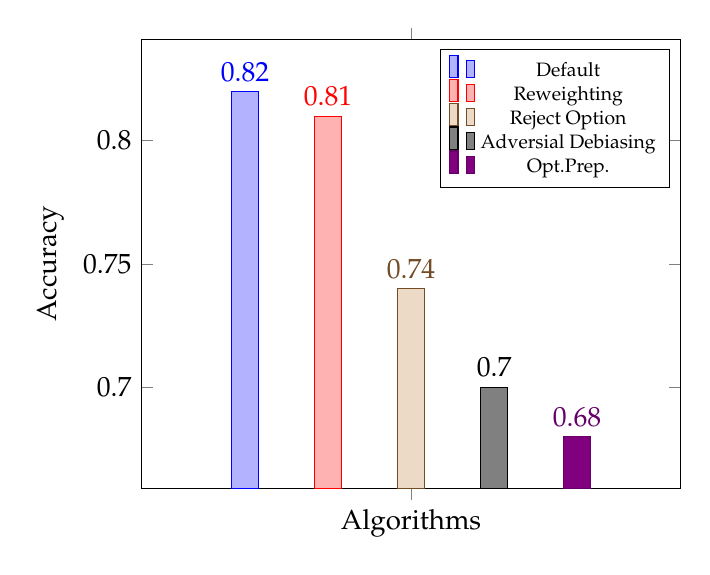
\begin{tikzpicture}
\begin{axis}[
    ybar=20pt,
    enlargelimits=0.15,
    legend style={font=\scriptsize,row sep=-0.1cm},
    ylabel={Accuracy},
    symbolic x coords={Algorithms},
    xtick=data,
    nodes near coords,
    nodes near coords align={vertical},
    ]
\addplot coordinates {(Algorithms,.82)};
\addplot coordinates {(Algorithms,.81)};
\addplot coordinates {(Algorithms,.74)};
\addplot coordinates {(Algorithms,.70)};
\addplot coordinates {(Algorithms,.68)};
\legend{Default,Reweighting,Reject Option,Adversial Debiasing,Opt.Prep.}
\end{axis}
\end{tikzpicture}
\caption{When fairness is detrimental to predictive performance.}\label{fig:Fairness}
\end{wrapfigure}
Our experience is that most of the fairness algorithms, including
adversarial debiasing   achieve fairness by damaging
predictive performance.  \fig{Fairness} shows that various fairness algorithms damage model accuracy to achieve fairness (tested on  Adult Census Income with protected attribute - "Sex")~\cite{IBM}. Note that,
compared to the performance of the default model,
many of the fairness operators results in large decreases in predictive performance.

Later in this proposal, we show that the performance decreases of \fig{Fairness} are optional.
Specifically, we show that if hyperparameter optimizers are asked to manage accuracy {\em and}
fairness, then it is possible to maintain predictive performance while also increase the fairness of the model
Those results are described in the next section.
 
Before going on, we note that there are there are many ways to measure ``fairness'' in a machine learning model.
We using the following definitions:
\bi
\item
 
 A label is called \textit{favorable label} if its  value corresponds to an outcome that gives an advantage to the receiver (e.g. being hired for a job, receiving a loan).
 \item
A \textit{protected attribute} is an attribute that divides a population into two groups that have difference in terms of benefit received  (e.g. race, sex, gender). These attributes are not universal, but are specific to application.
 \item
\textit{Group fairness} is the goal that based on the protected attribute, privileged and unprivileged groups will be treated similarly. 
 \item
\textit{Individual fairness} is the goal of similar individuals will receive similar outcomes.  For
this current proposal, we focus on  Group fairness only.
 \item
{\em Bias} is a systematic error~\cite{bias_systemetic}
and our main concern is unwanted bias that puts privileged groups at a systematic advantage and unprivileged groups at a systematic disadvantage. 
\ei

A \textit{fairness metric} is a quantification of unwanted bias in models or training data~\cite{IBM}. 
For the experiments reported later in this paper, we use two such metrics:
\bi
\item \textbf{Equal Opportunity Difference(EOD)}:    delta of true positive rates in unprivileged \& privileged groups~\cite{IBM}. 
\item \textbf{Average Odds Difference(AOD)}: The average delta in false positive rates and true positive rates between privileged and unprivileged groups~\cite{IBM}.
\ei
A value of 0 implies that both groups have equal benefit, a value lesser than 0 implies higher benefit for the privileged group and a value greater than 0 implies higher benefit for the unprivileged group. In this study, we have taken absolute value of these metrics. 


% \subsection{About Hyperparameter Optimization}\label{tion:hbo}
% The previous section described fairness metrics.
% This section describes automatic methods for altering machine
% learners in order to generate   models that perform well on those metrics. 
  
% Every machine learning algorithm has ``magic'' control parameters. For example:
% \bi
% \item Random forests have a hyperparameter that specifics how many trees in the forest;
% \item 
% When a support vector machines use some kernel and that kernel is specified by a set of parameters, 
% then that kernel and its settings are hyperparameters.
% \item
% When a neural nets use a certain network topology that includes $X$ nodes per layer, then than topology and that value $X$ are hyperparameters. 
% \ei

% \begin{wraptable}{r}{3in}
% \small
% \begin{tabular}{|p{2.9in}|}\hline
% \rowcolor{gray!20}
% If TN, FN, FP, TP are  true negatives, false negatives, false positives,  true positives, then:
% \bi
% \item
% {\em prec} = Precision = TP/(TP+FP) which  measures  the percentage of the predicted class that are actual members of the target class.
% \item 
% {\em pd} = Recall = TP/(TP+FN) which measures the percentage of the actual targets that are predicted to be targets.
% \item
% {\em pf} = False Alarms = FP/(FP+TN), the percentage of the non-target artifacts that are reported as part of the target class;  
% \ei\\\hline
% \end{tabular}
% \caption{Standard   machine learning metrics.}\label{tbl:metrics}
% \end{wraptable} ``Off of the shelf''
%  learners   come
% with   defaults for  control parameters, which may be sub-optimal. For example,
% in the  distance function  $d(x,y,p)=\left(\sum_i (x_i-y_i)^p\right)^{1/p}$,
% a standard default is $p=2$ (i.e. Euclidean distance). Yet Agrawal et al.~\cite{agrawal2017better}  found that
% $p>2$ worked much better for their processing. 



% Hyperparameter optimizers are automatic tools to find better control parameters~\cite{biedenkapp2018hyperparameter}~\cite{franceschi2017forward}. 
% This is done by experimenting with adjustments to the control parameters of a learner. 
% When done using 21st century optimizers (e.g. NSGA-2~\cite{deb00afast}, IBEA~\cite{Zitzler04indicator-basedselection}, MOEA/D~\cite{zhang07}, FLASH~\cite{nair18}), it is now possible to optimizer for multiple goals (even when they are competing). 
%  PI Menzies has had much success  with   
% hyperparameter optimizers  to automatically determine which learner to use, and what settings to apply to those learners~\cite{fu2016tuning,chen2017riot,nair2017flash,agrawal2017better,fu2017revisiting,nair2017using,mathew2017shorter,nair2017faster,chen2017beyond,nair2016accidental,fu2016differential,chen2016sampling,agrawal2016wrong,agrawal2018better}.
% In all that work, the optimizers sought ways to improve standard performance measures
% like recall, precision, and false alarm (defined in \tbl{metrics}).
% In this  proposal, we 
% we will  explore hyperparamter optimizers that seek to manage these standard performance
% measures {\em as well as } the fairness metrics described above.


% There are  many ways to implement hyperparameter optimizers.
% \textit{Grid search}~\cite{bergstra2011algorithms} 
%   creates   
% $C$ nested for-loops to explore   $C$ control parameters.  Bergstra et al. depreciate grid search arguing that (a)~the best hyperparameters are usually found within a very small region of the total space;  and (b)~a grid search that is fine-grained enough to find that region for any learner and any data set would be very slow indeed~\cite{bergstra2011algorithms}

 


% \begin{figure} 
% \small
% \begin{center}
% \begin{tabular}{|r|p{5in}|}
% \hline
%  &\cellcolor{gray!20}
% Start with data $D$ and a small sample $S \subset D$ of, say, 20 examples,
% labelled with their  goals values.
% \\
% LOOP:&Using $S$ and a  data miner, build one model per goal.  In standard BPO, 
% a Gaussian Process Model (GPM) is used for this step. FLASH replaces
% GPM with CART decision trees
% so the resulting systems
% scales to much larger problems; and the learned model is simple and succinct
% enough to show to business users~\cite{nair2017flash}. 
% \\

% &\cellcolor{gray!20}Using those models, guess goal values for  
% $D-S$.
% \\
% &Select   $X \in D-S$ with the ``best''  guesses.  BPO
% collects information only on the next most informative example. In our current favorite
% implementation~\cite{nair2017flash} we use a random project method to find the $X$ that most maximizes
% our goals (across a wide range of possible weighting questions).
% \\ 
% &\cellcolor{gray!20}Evaluate  $X$s' goals. 
% \\
% &
% Let $S=S+X$.  
% \\
 
% &\cellcolor{gray!20} Go to ``LOOP:''
% \\\cline{2-2} \hline
% \end{tabular}
% \end{center}
% \caption{     Hyperparameter optimizer with FLASH~\cite{nair18}.}\label{tbl:flash}
% \end{figure}
 
% ~\textit{Random search}~\cite{bergstra2012random} sets up ranges  of hyperparameter values and select random combinations to train the model and evaluate. 
% There are many such methods including those that use genetic algorithms
% such as  NSGA-2~\cite{deb00afast}, IBEA~\cite{Zitzler04indicator-basedselection}, or MOEA/D~\cite{zhang07}. While an effective strategy, random search may require
% too many evaluations to be practice.

% In contrast to Grid or Random search, \textit{Bayesian optimization}~\cite{pelikan1999boa} keeps track of past evaluation results and use them to build a probabilistic model mapping hyperparameters to a probability of a score on the objective function \cite{Will_Koehrsen}. This probabilistic model is called ``surrogate'' for the objective function. The idea is to find the next set of hyperparameters to evaluate on the actual objective function by selecting hyperparameters that perform best on the surrogate function.

% \textit{Sequential model-based optimization (SMBO)} \cite{hutter2011sequential} is a formalization of Bayesian optimization. It runs trials one by one sequentially, each time trying better hyperparameters using Bayesian reasoning and updating the surrogate model \cite{Will_Koehrsen}. 
% Recently~\cite{nair18}, we have had   success  
% an SMBO algorithm called  FLASH,   The  pseudo code of \tbl{flash}     shows how FLASH  minimizes
%   evaluating different tunings
%   by   collecting information on only the most interesting examples.


% % \textbf{FLASH: A Fast Sequential Model-Based Method:}
% % Nair et al. \cite{8469102} proposed a fast SMBO approach called FLASH for multiobjective optimization. FLASH's acquisition function uses Maximum Mean. Maximum Mean returns the sample (configuration) with the highest expected (performance) measure. FLASH models each objective as a separate performance (CART) model. Because the CART model can be trained for one performance measure or dependent value. Nair reports that FLASH runs orders of magnitude faster than NSGA-II, but that was for software configuration problems. This work is the first study to try using  FLASH to optimize for learner performance while at the same time improving fairness.



% % the worst of which is 
% % a {\em grid search} which creates  try many combinations of $C$ parameters
% % using $C$ nested for-loops~\cite{Bergstra:2012}.
% % Bergstra et al. depreciates grid search arguing that (a)~the best hyperparameters are found
% % within a very small region of the total space; and (b)~a grid search that is fine-grained
% % enough to find that  region for any learner and any dataset would be very slow indeed~\cite{Bergstra:2012}.

% % require thousands to millions of executions of a learner. 

% % Differential evolution is just one in a large suite of possibly useful stochastic optimization algorithms
% % that PI Menzies has used to improve different data mining tasks~\cite{fu2016tuning,chen2017riot,nair2017flash,agrawal2017better,agrawal2017better,fu2017revisiting,nair2017using,mathew2017shorter,nair2017faster,chen2017beyond,nair2016accidental,fu2016differential,chen2016sampling,agrawal2016wrong}.
% % For example 

  
  
% \begin{table}
% \centering
% \footnotesize
% \caption{Optimizing just for fairness.  
% Change in  Recall and False alarm before and after bias mitigation. Gray= improvement; black= damage.
% From~\cite{Chakraborty}.}
% \label{tbl:fairness_cost}
% \begin{tabular}{|l|c|c|r|r|r|r|}\cline{4-7}
 
% \multicolumn{3}{c}{~}
% &\multicolumn{2}{|p{.7in}}{{\em larger} values are {\em better}}&
% \multicolumn{2}{|p{.8in}|}{{\em smaller} values are {\em better}}\\
% \rowcolor[HTML]{C0C0C0} 
% \cellcolor[HTML]{C0C0C0} & 
% \multicolumn{1}{l|}{\cellcolor[HTML]{C0C0C0}} & 
% \multicolumn{1}{l|}{\cellcolor[HTML]{C0C0C0}} & \multicolumn{2}{c|}{\cellcolor[HTML]{C0C0C0}Recall} & \multicolumn{2}{c|}{\cellcolor[HTML]{C0C0C0}False alarm} \\ \cline{4-7} 


% \rowcolor[HTML]{C0C0C0} 
% \multirow{-2}{*}{\cellcolor[HTML]{C0C0C0}Algorithm} & \multicolumn{1}{l|}{\multirow{-2}{*}{\cellcolor[HTML]{C0C0C0}Dataset}} & \multicolumn{1}{l|}{\multirow{-2}{*}{\cellcolor[HTML]{C0C0C0}\begin{tabular}[c]{@{}l@{}}Protected \\ Attribute\end{tabular}}} & \multicolumn{1}{c|}{\cellcolor[HTML]{C0C0C0}Before} & \multicolumn{1}{l|}{\cellcolor[HTML]{C0C0C0}After} & \multicolumn{1}{c|}{\cellcolor[HTML]{C0C0C0}Before} & \multicolumn{1}{l|}{\cellcolor[HTML]{C0C0C0}After} \\ \hline
% \multicolumn{1}{|c|}{} &  & Sex & 83 & \cellcolor[HTML]{FFFFFF}{\color[HTML]{333333} 83} & 34 & \cellcolor[HTML]{333333}{\color[HTML]{FFFFFF} 43} \\ \cline{3-7} 
% \multicolumn{1}{|c|}{} & \multirow{-2}{*}{Adult} & Race & 83 & \cellcolor[HTML]{FFFFFF}{\color[HTML]{333333} 83} & 34 & \cellcolor[HTML]{333333}{\color[HTML]{FFFFFF} 35} \\ \cline{2-7} 
% \multicolumn{1}{|c|}{} &  & Sex & 60 & 60 & \cellcolor[HTML]{FFFFFF}{\color[HTML]{333333} 27} & \cellcolor[HTML]{333333}{\color[HTML]{FFFFFF} 29} \\ \cline{3-7} 
% \multicolumn{1}{|c|}{} & \multirow{-2}{*}{Compas} & Race & 62 & \cellcolor[HTML]{333333}{\color[HTML]{FFFFFF} 61} & \cellcolor[HTML]{FFFFFF}{\color[HTML]{333333} 27} & \cellcolor[HTML]{333333}{\color[HTML]{FFFFFF} 34} \\ \cline{2-7} 
% \multicolumn{1}{|c|}{} &  & Sex & 70 & \cellcolor[HTML]{333333}{\color[HTML]{FFFFFF} 69} & \cellcolor[HTML]{FFFFFF}66 & \cellcolor[HTML]{333333}{\color[HTML]{FFFFFF} 77} \\ \cline{3-7} 
% \multicolumn{1}{|c|}{\multirow{-6}{*}{Reweighing}} & \multirow{-2}{*}{German} & Age & 70 & \cellcolor[HTML]{C0C0C0}71 & \cellcolor[HTML]{FFFFFF}66 & \cellcolor[HTML]{C0C0C0}25 \\ \hline
%  &  & Sex & 83 & \cellcolor[HTML]{333333}{\color[HTML]{FFFFFF} 76} & \cellcolor[HTML]{FFFFFF}34 & \cellcolor[HTML]{333333}{\color[HTML]{FFFFFF} 35} \\ \cline{3-7} 
%  & \multirow{-2}{*}{Adult} & Race & 83 & 83 & \cellcolor[HTML]{FFFFFF}34 & \cellcolor[HTML]{333333}{\color[HTML]{FFFFFF} 37} \\ \cline{2-7} 
%  &  & Sex & 60 & 60 & \cellcolor[HTML]{FFFFFF}27 & \cellcolor[HTML]{333333}{\color[HTML]{FFFFFF} 29} \\ \cline{3-7} 
%  & \multirow{-2}{*}{Compas} & Race & 62 & \cellcolor[HTML]{C0C0C0}{\color[HTML]{333333} 65} & \cellcolor[HTML]{FFFFFF}27 & \cellcolor[HTML]{333333}{\color[HTML]{FFFFFF} 29} \\ \cline{2-7} 
%  &  & Sex & 70 & \cellcolor[HTML]{333333}{\color[HTML]{FFFFFF} 69} & \cellcolor[HTML]{FFFFFF}66 & \cellcolor[HTML]{C0C0C0}{\color[HTML]{333333} 36} \\ \cline{3-7} 
% \multirow{-6}{*}{\begin{tabular}[c]{@{}l@{}}Optimized \\ Pre-\\ processing\end{tabular}} & \multirow{-2}{*}{German} & Age & 70 & \cellcolor[HTML]{333333}{\color[HTML]{FFFFFF} 68} & \cellcolor[HTML]{FFFFFF}66 & \cellcolor[HTML]{C0C0C0}{\color[HTML]{333333} 58} \\ \hline
%  &  & Sex & 82 & \cellcolor[HTML]{C0C0C0}83 & 35 & \cellcolor[HTML]{333333}{\color[HTML]{FFFFFF} 42} \\ \cline{3-7} 
%  & \multirow{-2}{*}{Adult} & Race & 82 & 82 & 35 & 35 \\ \cline{2-7} 
%  &  & Sex & 60 & 60 & 27 & \cellcolor[HTML]{333333}{\color[HTML]{FFFFFF} 28} \\ \cline{3-7} 
%  & \multirow{-2}{*}{Compas} & Race & 60 & 60 & 27 & \cellcolor[HTML]{333333}{\color[HTML]{FFFFFF} 28} \\ \cline{2-7} 
%  &  & Sex & 70 & \cellcolor[HTML]{C0C0C0}75 & 66 & \cellcolor[HTML]{C0C0C0}61 \\ \cline{3-7} 
% \multirow{-6}{*}{\begin{tabular}[c]{@{}l@{}}Adversial\\ Debiasing\end{tabular}} & \multirow{-2}{*}{German} & Age & 70 & \cellcolor[HTML]{333333}{\color[HTML]{FFFFFF} 69} & 50 & \cellcolor[HTML]{333333}{\color[HTML]{FFFFFF} 72} \\ \hline
%  &  & Sex & 83 & \cellcolor[HTML]{333333}{\color[HTML]{FFFFFF} 24} & 34 & \cellcolor[HTML]{C0C0C0}05 \\ \cline{3-7} 
%  & \multirow{-2}{*}{Adult} & Race & 83 & \cellcolor[HTML]{333333}{\color[HTML]{FFFFFF} 28} & 34 & \cellcolor[HTML]{C0C0C0}04 \\ \cline{2-7} 
%  &  & Sex & 62 & \cellcolor[HTML]{C0C0C0}{\color[HTML]{333333} 97} & 27 & \cellcolor[HTML]{333333}{\color[HTML]{FFFFFF} 89} \\ \cline{3-7} 
%  & \multirow{-2}{*}{Compas} & Race & 62 & \cellcolor[HTML]{C0C0C0}{\color[HTML]{333333} 68} & 27 & \cellcolor[HTML]{333333}{\color[HTML]{FFFFFF} 38} \\ \cline{2-7} 
%  &  & Sex & 70 & \cellcolor[HTML]{C0C0C0}{\color[HTML]{333333} 96} & 66 & \cellcolor[HTML]{333333}{\color[HTML]{FFFFFF} 95} \\ \cline{3-7} 
% \multirow{-6}{*}{\begin{tabular}[c]{@{}l@{}}Reject\\ Option\end{tabular}} & \multirow{-2}{*}{German} & Age & 70 & 70 & 66 & 66 \\ \hline
%  &  & Sex & 83 & \cellcolor[HTML]{333333}{\color[HTML]{FFFFFF} 78} & 39 & \cellcolor[HTML]{333333}{\color[HTML]{FFFFFF} 40} \\ \cline{3-7} 
%  & \multirow{-2}{*}{Adult} & Race & 83 & \cellcolor[HTML]{333333}{\color[HTML]{FFFFFF} 78} & 39 & \cellcolor[HTML]{C0C0C0}35 \\ \cline{2-7} 
%  &  & Sex & 65 & \cellcolor[HTML]{333333}{\color[HTML]{FFFFFF} 63} & 38 & \cellcolor[HTML]{333333}{\color[HTML]{FFFFFF} 40} \\ \cline{3-7} 
%  & \multirow{-2}{*}{Compas} & Race & 65 & 65 & 38 & \cellcolor[HTML]{333333}{\color[HTML]{FFFFFF} 39} \\ \cline{2-7} 
%  &  & Sex & 74 & \cellcolor[HTML]{333333}{\color[HTML]{FFFFFF} 72} & 20 & \cellcolor[HTML]{333333}{\color[HTML]{FFFFFF} 33} \\ \cline{3-7} 
% \multirow{-6}{*}{\begin{tabular}[c]{@{}l@{}}FLASH\\ optimizes for\\ AOD \& EOD\end{tabular}} & \multirow{-2}{*}{German} & Age & 74 & \cellcolor[HTML]{333333}{\color[HTML]{FFFFFF} 68} & 20 & \cellcolor[HTML]{333333}{\color[HTML]{FFFFFF} 45} \\ \hline
% \end{tabular}
% \end{table}
 

\section{Preliminary Results}\label{preliminary}


Recent studies have shown that hyperparameter optimization can achieve better performance than using ``off-the-shelf'' configurations in several research areas in software engineering, e.g., software effort estimation\cite{xia2018hyperparameter} and software defect prediction\cite{osman2017hyperparameter}. We are first to apply hyperparameter optimization in software fairness domain~\cite{Chakraborty}.

%  \subsection{  Hyperparameter Optimization \& Fairness}\label{tion:ms}
% \tbl{fairness_cost} show what happens when the above seven steps
% of FLASH 
% are applied to fairness.
% \tbl{fairness_cost} applies various fairness operators (taken from   github.com/IBM/AIF360) to protect various attributes
% within the the Adult, Compas, and German data sets (these are standard data sets used for experimentation in this field).


% In \tbl{fairness_cost}, gray denotes an improvement in predictive
% performance and black denotes worse predictive performance. 
% The last few lines  of     \tbl{fairness_cost}  shows FLASH optimizing in order to minimize
% the absolute value of both EOD {\em and} AOD (the fairness metrics described in the last section).
% In those results, we asked FLASH to minimize the
% absolute value of EOF and AOD. To do this,
% we let FLASH tune four hyperparameters for two learners:
% \bi
% \item Logistic regression (which learns an equation):
% \bi
% \item C: Inverse of regularization strength where smaller values specify stronger regularization.
% \item
% penalty: Used to specify the norm used in the penalization applied to the model.
% \item solver: Algorithm to use in the optimization problem
% \item maxiter: Maximum number of iterations taken for the solvers to converge.
% \ei
% \item
% CART (which learns an decision tree):
% \bi
% \item criterion: The function to measure the quality of a split.
% \item splitter: The strategy used to choose the split at each node.
% \item minsamplesleaf: The minimum number of samples required to be at a leaf node. A split point at any depth will only be considered if it leaves at least certain number of training samples in each of the left and right branches.
% \item minsamplessplit: The minimum number of samples required to split an internal node.
% \ei
% \ei
% In the FLASH results, 
% the two things to observe from
% \tbl{fairness_cost}  are:
% \bi
% \item
% Firstly,
% there are many  black entries; i.e.
% applying the fairness operators has negative impact on predictive performance.
% Some of the changes in  in performance are negligible (e.g. false alarms changing from 27 to 28).
% But in other cases, the impact of applying the fairness operators is truly alarming, particularly for the false alarm rates (e.g  for ``reject option'', we can see false alarms increasing from 27\% to 89\% in some cases).

% This negative impact of fairness operators on performance prowess is somewhat alarming. Historically,
% it was the original motivator for this research.
% \item
% Secondly, 
% of all the fairness operators, FLASH has the most black entries
% in both recall and false alarm.  
% It is easy to explain, and to fix, FLASH's poor performance in   \tbl{fairness_cost}.
% Hyperparameter optimizers are servants that follow our instructions. In  \tbl{fairness_cost}, we told to
% FLASH to optimize for fairness, but not to care about recall and false alarms. Not surprisingly, this lead
% to FLASH generating models with  poor predictive prowess.
% \ei


% \begin{table}[!t]
% \centering
% \footnotesize
% \caption{Optimizing for fairness, lower false alarm and higher recall. Gray=improvement; black=damage.
% Note that, compared to Table~\ref{tbl:fairness_cost}, there is far less damage. From~\cite{Chakraborty}.}
% \label{tbl:multiobjective_results}
% \begin{tabular}{|l|l|c|r|r|r|r|r|r|>{\columncolor[HTML]{FFFFFF}}r |r|}
% \cline{4-11}
 
% \multicolumn{3}{c}{~}
% &\multicolumn{2}{|p{.7in}}{{\em larger} values are {\em better}}&
% \multicolumn{2}{|p{.8in}|}{{\em smaller} values are {\em better}}&
% \multicolumn{4}{c|}{{\em smaller} values are {\em better}} \\

% \hline
% \cellcolor[HTML]{C0C0C0} & \cellcolor[HTML]{C0C0C0} & \multicolumn{1}{l|}{\cellcolor[HTML]{C0C0C0}} & \multicolumn{2}{c|}{\cellcolor[HTML]{C0C0C0}Recall} & \multicolumn{2}{c|}{\cellcolor[HTML]{C0C0C0}\begin{tabular}[c]{@{}c@{}}False \\ alarm\end{tabular}} & \multicolumn{2}{c|}{\cellcolor[HTML]{C0C0C0}AOD} & \multicolumn{2}{c|}{\cellcolor[HTML]{C0C0C0}EOD} \\ \cline{4-11} 
% \multirow{-2}{*}{\cellcolor[HTML]{C0C0C0}Model} & \multirow{-2}{*}{\cellcolor[HTML]{C0C0C0}Dataset} & \multicolumn{1}{l|}{\multirow{-2}{*}{\cellcolor[HTML]{C0C0C0}\begin{tabular}[c]{@{}l@{}}Protected \\ Attribute\end{tabular}}} & \multicolumn{1}{c|}{\cellcolor[HTML]{C0C0C0}Before} & \cellcolor[HTML]{C0C0C0}After & \multicolumn{1}{c|}{\cellcolor[HTML]{C0C0C0}Before} & \cellcolor[HTML]{C0C0C0}After & \multicolumn{1}{c|}{\cellcolor[HTML]{C0C0C0}Before} & \cellcolor[HTML]{C0C0C0}After & \multicolumn{1}{c|}{\cellcolor[HTML]{C0C0C0}Before} & \cellcolor[HTML]{C0C0C0}After \\ \hline
% \multicolumn{1}{|c|}{} &  & Sex & 83 & \cellcolor[HTML]{333333}{\color[HTML]{FFFFFF} 78} & 39 & \cellcolor[HTML]{C0C0C0}{\color[HTML]{333333} 32} & 31 & \cellcolor[HTML]{C0C0C0}09 & 49 & \cellcolor[HTML]{C0C0C0}15 \\ \cline{3-11} 
% \multicolumn{1}{|c|}{} & \multirow{-2}{*}{Adult} & Race & 83 & \cellcolor[HTML]{333333}{\color[HTML]{FFFFFF} 80} & 39 & \cellcolor[HTML]{C0C0C0}{\color[HTML]{333333} 31} & 14 & \cellcolor[HTML]{C0C0C0}04 & 22 & \cellcolor[HTML]{C0C0C0}08 \\ \cline{2-11} 
% \multicolumn{1}{|c|}{} &  & Sex & 65 & 65 & \cellcolor[HTML]{FFFFFF}{\color[HTML]{333333} 38} & 38 & 24 & 24 & 29 & 29 \\ \cline{3-11} 
% \multicolumn{1}{|c|}{} & \multirow{-2}{*}{Compas} & Race & 65 & 65 & \cellcolor[HTML]{FFFFFF}{\color[HTML]{333333} 38} & 38 & 12 & 12 & 16 & 16 \\ \cline{2-11} 
% \multicolumn{1}{|c|}{} &  & Sex & 74 & 74 & \cellcolor[HTML]{FFFFFF}2 & 2 & 12 & 12 & 04 & 04 \\ \cline{3-11} 
% \multicolumn{1}{|c|}{\multirow{-6}{*}{\begin{tabular}[c]{@{}c@{}}Logistic\\ regression\end{tabular}}} & \multirow{-2}{*}{German} & Age & 74 & 74 & \cellcolor[HTML]{FFFFFF}2 & 2 & 44 & 44 & 08 & 08 \\ \hline
%  &  & Sex & 83 & 83 & \cellcolor[HTML]{FFFFFF}36 & 36 & \cellcolor[HTML]{FFFFFF}29 & 29 & 46 & 46 \\ \cline{3-11} 
%  & \multirow{-2}{*}{Adult} & Race & 83 & 83 & \cellcolor[HTML]{FFFFFF}36 & 36 & \cellcolor[HTML]{FFFFFF}14 & 14 & 24 & 24 \\ \cline{2-11} 
%  &  & Sex & 65 & 65 & \cellcolor[HTML]{FFFFFF}35 & 35 & \cellcolor[HTML]{FFFFFF}25 & 25 & 29 & 29 \\ \cline{3-11} 
%  & \multirow{-2}{*}{Compas} & Race & 65 & 65 & \cellcolor[HTML]{FFFFFF}35 & 35 & \cellcolor[HTML]{FFFFFF}23 & 23 & 26 & 26 \\ \cline{2-11} 
%  &  & Sex & 74 & 74 & \cellcolor[HTML]{FFFFFF}5 & \cellcolor[HTML]{333333}{\color[HTML]{FFFFFF} 29} & \cellcolor[HTML]{FFFFFF}15 & \cellcolor[HTML]{C0C0C0}1 & 14 & \cellcolor[HTML]{C0C0C0}3 \\ \cline{3-11} 
% \multirow{-6}{*}{CART} & \multirow{-2}{*}{German} & Age & 74 & 74 & \cellcolor[HTML]{FFFFFF}5 & \cellcolor[HTML]{333333}{\color[HTML]{FFFFFF} 29} & \cellcolor[HTML]{FFFFFF}60 & \cellcolor[HTML]{C0C0C0}53 & 21 & \cellcolor[HTML]{C0C0C0}7 \\ \hline
% \end{tabular}
% \end{table}

% \subsection{  Four Goal Optimization}\label{tion:ms}
% To fix FLASH, all we need to do is ask it to optimize for four goals: improve EOD {\em and} improve AOD {\em and} minimize
% false alarms {\em and} maximize recall. The results of this four goal optimization run is shown in
% \tbl{multiobjective_results}. Note that, in these results,
% there are far fewer  black cells \tbl{multiobjective_results} than in  \tbl{fairness_cost}; i.e. 
% if   our optimizer know
% all the goals that matter, then it can generate better solutions across those spaces of goals.
% Also, 
% unlike \fig{Fairness}, we see that with 4-goal hyperparameter optimization, fairness need not be detrimental
% to   predictive performance since, 
% as seen in \tbl{multiobjective_results}:
% \bi
% \item
% Using logistic regression, in the Adult data set, we can improve AOD and EOD for sex and race by almost three
% times.
% \item Even larger improvements are available, perhaps using other learners.
% For example, using CART, in the German data set, for the sex attributes,   EOD and AOD are improved five to fifteen times.
% \ei
% Improving fairness might require switching the learning algorithm. As evidence of that,
% note that:
% \bi
% \item
% Logistic regression   improves
% fairness in the Adult data set, not mot for German.
% \item
% For that data set, to improve fairness, we need to use CART.
% \ei
% This last finding is particularly troubling for Model Stores. Usually, the models in Model Stores are hardwired
% to a specific learner
% but \tbl{multiobjective_results} indicates that maintaining fairness can requre exploring a wider range of  options. 

 


\section{Open Issues}\label{open}

 
% The goal of this proposal is to   make hyperparameter optimization for fairness so fast and effective
% that it can routinely be applied to model generation (via data miners).

\noindent
The above results are promising, but incomplete, for several reasons:
\bi
\item
The above results only assess the success
of optimizing-for-fairness via fairness measures (EOD and AOD) and predictive prowess (recall
and false alarm). Another important assessment criteria is the 
{\em time} and associated  {\em CPU cost} of generating those models. 
Even our most optimized optimizer (FLASH) needs to execute learners 20 to 100 times.
That is, when exploring just one learner, hyperparameter optimization can take two
orders of magnitude more CPU to reach its conclusions.
This an important point since,
as stated in the introduction, 
any method requiring excessive addition CPU is contraindicated for Model Store models.
Within a Model Store, users pay for access to the machine learner
as well as the CPU required to run, test, and possibly tune, that model.
That is, the users
purchasing those models must foot the bill for the associated CPU costs.
If Model Store clients have a choice of models, and some are orders of magnitude cheaper to buy than others
(i.e. the ones that do not use hyperparameter optimization), then the natural tendency of consumers
will be to favor the cheaper product (even if that cheaper product is more unfair).
\item
The  above results make no use of any prior experience with 
applying   optimization-for-fairness to a learner. This is a major deficiency in our prior work since,
in the context of Model Stores, similar models would be generated many times (whenever multiple
users hired and applied the same Model Store app). In theory, prior optimization
experience might be used to speed-up any subsequent optimization study.  
\item
The above results are based on only a few data sets--
so we need to explore models.
Of particular importance here is the
last result mentioned above; i.e. that sometimes the best hyperparameter optimization
is achieved via switching learners.  Theoretically, if we studied enough data sets and enough learners, we might find that some small set of learners are always
generating the best optimize-for-fairness results. If this were true then this would significantly reduce to the computational cost of hyperparameter optimization for fairness (since any optimize-for-fairness study would have to try  fewer   learners). 
\item
The above results
are based on binary classifiers with simplistic measures for predictive prowess
(just the measures of \tbl{metrics}). There are many more measures we have yet to explore. For example, consider the {\em Hospital  Readmission} model described on \tion{problem}. 
For that model, predictive prowess means minimizing the time/cost of hospitalization
while also minimizing the probability of negative medical outcomes (a.k.a. death).  
\item
In terms of \tbl{multicol}, the above results just explore one kind of fairness operator;
specifically the  ``in-processing'' kind of fairness operator that adjusts the learning process.
There are other kinds of fairness operators that need to be explored such as pre- and post- processing operators. 
\item
Section~\tion{ms} mentions about the hyperparameter options explored as part of using optimizer but the hyperparameter optimization space of these algorithms are much more vast. Exploring these options will require vast amount of CPU resources. Thus we will require to make a trade-off between exploring the extend of hyperparameter space and cost awareness of the models.
\item
Quality of data used in training can impact the predictive power of model in multiple ways which is why data preprocessing is a major area of research. There are various techniques that can be applied and utilized to improve predictive results such as removals of outliers, data balancing by minority oversampling or majority down sampling, attribute section, data weighting etc. All these different techniques need to be explored to achieve desired performance. 

\ei

\newcommand{\head}[1]{\noindent{\bf \underline{#1}}:}

\section{Research Plan}\label{tion:plan}


\noindent
To address these open issues, our research plan  has five parts:
\be
\item
{\bf Initial Set-up}:
In steps
one,two,three and four, we conduct some background studies
to collect the data needed to assess the results of steps five and beyond.
\item
{\bf (re)Building {\IT}}:
Next, in steps five to eight, we explore  the three kinds
of fairness operators described in \tbl{multicol}; i.e. pre-, in- and post- processing of machine learners. The tool we call {\IT} is a combination
of these three operators, plus a set of heuristics telling us
when to use which operator.
\item
{\bf Extend to Multiple Learners:}
Initially, for steps one to eight, 
we will assume that the machine learner is not
to be changed (so we will use whatever learner appears is found in  the Model Store
application). But after that, we will loop back though steps one to eight
allowing the optimizer-for-fairness to switch learners if it wants
to. By doing this, we will (a)~get some
quick initial results; then
(b)~be able to assess the value of optimize-for-fairness using
single vs multiple learners.
\ei
Finally, running in parallel across the other parts, we have two other important activities:
\begin{enumerate}[topsep=0pt,bottomsep=0pt,itemsep=0,leftmargin=*]
    \setlength{\itemsep}{0pt}
    \setlength{\parskip}{0pt}
    \setlength{\parsep}{0pt}    
    \addtocounter{enumi}{3}
\item
{\bf Packaging and Sharing of Methods:}
Whenever we have evidence that we can significantly reduce
the CPU cost of optimization-as-fairness, we will (a)~package up our software as a public domain Python package; (b)~reach out to Model Store managers and app store developers to share our results with them.
\item
{\bf Comparisons with other Fairness Research}: Fairness research is a very active research area. 
Hence, we foresee that over the course of this grant, many  fairness operators will be published.
Accordingly, it is important that what results obtained in this grant are compared with the state-of-the-art
in the fairness literature. 
\end{enumerate}
For details notes on all these five parts, see below.

 \subsection{Part1: Initial Set-up}
 
\subsubsection{Step 1. Build ``Lab Rats''}\label{tion:labrat}
In this step, we will build our  ``lab rats''; i.e. models that will be explored using optimziation-for-fairness.
In this first step, we will  repeat the analysis 
of \tion{problem}, but at a much larger scale; i.e. for the hundreds of known models
in the Model Stores. 
We would then study those models in order to generate
a catalogue of   (a)~the available models;  (b)~lists of developers (for the Model Store apps) and~(c)~lists of data/learners used; (d)~list attributes within each model that we wish to protect (e.g. age, race, gender, income, etc). 
Using this list we would 
\bi
\item Extend our definitions of predictive prowess beyond the list of \tbl{metrics}.
For example, to repeat the example
offered above,
the  {\em Hospital  Readmission} model described in \tion{problem}
might need to minimize
the time/cost of hospitalization
while also minimizing the probability of negative medical outcomes.
Other models may have other definitions of ``good'' predictions: e.g. safety-critical
apps may allow large false negative results, just as long as the recall results
are exception.
\item
Contact the Model Store app developers, informing them of
our research and asking them to contribute data and models. There are many ways we could contact them,
the easiest being to leave remarks in the comments sections of the Model Store.
We would negotiate with them
a non-disclosure agreement with the following clause.
If we find fairness issues in their models, they will be the first to be told.
After that, that result will be embargoed for 12 months such that no outside
is aware of fairness issues in that model for one year after we notify the Model
Store app developers.
\item
Look for models that we can recreate, within our own lab, using public domain
data and public domain learners. Our preliminary analysis of the Model Stores
suggests that there are numerous such models.
\ei
Just to speak to the practicality of the last point,
we note that  a new trend within  Model Stores
is to include sample data with the Model Store app  (e.g. in the AWS marketplace,
see 
{\em  Attribution prediction, Medical no show prediction, Credit default prediction})
 
 
 \newenvironment{success}[1]{ 
 \vspace{-1mm}
 \centerline\noindent\begin{minipage}{.9\linewidth}
    \begin{center}
    \arrayrulecolor{black}
    \begin{tabular}{|p{0.95\linewidth}|}\hline
         \rowcolor{gray!20}
         {\bf Success criteria for ``#1''}}{
    \\\hline\end{tabular}\end{center}\end{minipage}\vspace{1mm}}
    
     
    
\begin{success}{Lab rats}
We know the range of models/learners/evaluation criteria
that exist in the current model stores. Further, we can access
for ourselves a sample of models/learners across that range.
\end{success}

 
\subsubsection{Step 2. Create baselines1 (no tuning)} Here, we will build models using off-the shelf defaults from the learners. 
Currently, we have ready access
to many   machine learning algorithms (see  www.kdnuggets.com/software/libraries.html) including the WEKA JAVA toolkit
and the Scikit-learn Python toolkit. All these learners expose their control parameters.
In this step we will build models using the default parameters then record the observed fairness levels (using EOD and AOD) and predictive prowess
(using success measures appropriate to different models: recall and false alarm where appropriate, and perhaps other measures for other models-- see point4 in the previous section).  


\begin{success}{Baselines1}
We can   execute
for ourselves, outside the Model Stores, many of the
  models available within the Model Stores. 
\end{success}

\subsubsection{Step 3. Create baselines2 (with tuning)} Applying
our standard methods; i.e.
we would conduct optimization-as-fairness
with a machine learning algorithm.  Initially, we will 
conduct those tunings using the FLASH~\cite{nair2017flash} sequential model-based
optimizer described in  \tbl{flash}. Note that while this
optimizer is one the current state-of-the-art algorithms in this field,
as mentioned above, it still requires 20 to 100 executions
of the data miner to achieve its optimization goals. Hence,
in later steps of this proposal, we will strive to reduce the
computational cost of running some new optimization-as-fairness
run via reusing the experience gained in older 
optimization-as-fairness
runs.


\begin{success}{Baseline2}
By comparing with Baseline1,
we can determine how much we can improve fairness without damaging predictive prowess using standard optimizers. Here ``improvement'' will be measured
via fairness measures like EOD and AOD and predictive prowess will be measured
using the performance measures found in Step1.
\end{success}


\subsubsection{Step 4. Cost awareness}\label{tion:costaware} Once the prior step is completed,
we will know the computational cost of optimization-as-fairness.
Using the cost models for the Model Stores, we can then determine the cost to the user of optimization-as-fairness. Using qualitative methods (surveys,
focused interviews), we will learn the   sensitivity of Model
Store users to the these costs. Note that to conduct these qualitative surveys, we will start by  posting  comments   of the review sections on
the   Model Stores. 

This research team has much prior experience with running such qualitative studies~\cite{Menzies:2013:DSS:2486788.2487048,Menzies:2015:ASA:2819009.2819229,Menzies:2016:ADS:2889160.2891047}.


\begin{success}{Cost awareness}
We can draw cost awareness curves showing how much additional
cost-to-use a model impacts the number of purchases of that model.
\end{success}

Once such curves are available, we can define the overall success criteria of this project. In our introduction we said that one of our goals was to apply optimization-for-fairness at    ``not much'' more CPU cost that   than learning without tuning.
By studying the ``knee'' in the cost awareness curves, we can define what
value we need to assign to ``not much''.


 \subsection{Part2: (re)Building {\IT}}
 We will loop through this section many times. Initially
 we will build version1 of {\IT}. Subsequently,
 we will revisit that code and rebuild it (to make a better
 version).

\subsubsection{Step 5. Pre-processing: ``Match''ing Old Tunings} %\label{tion:plan}

 In this step we will
explore pre-processing using   {\bf Match}; i.e.   given $T$ prior tunings and  new data,  run the tuning $T_i$  see in similar prior data.
This approach assumes such prior tunings exists which, in the case
of Model Stores, is quite possible\footnote{When many users
rent and tune the same Model Store app, then the results of 
those tunings will be known to the Model Store app. If these tunings
are cached, then
they could be reused to simplify future tunings.}.
{\bf Match} is common industrial practice~\cite{dlreuse}, particularly
in the deep learning community where training is so lengthy and 
expensive. The black art in {\bf Match} is to select which prior
tuning is best for a new data set. Recently,   Truede and Wagner   added
  some clarity to the black art
  processing of matching to prior tunings~\cite{treude2018per}. They extracted featured from different data sets and used a decision tree learner to predict which prior tuning set
was best for new data:
The obvious advantage of this approach is ``zero cost tuning''; i.e. 
useful tunings can be discovered with no new experimentation. But the
 obvious disadvantages of this approach are:
\bi
\item {\em Closest, but not close enough:} ``Match'' can find the nearest
tuning from the space of old tunings, which is not necessarily
the same thing as the ``best'' tuning. 

\item {\em Negative transfer:} Pan et al.~\cite{Pan2010A}
warn that reusing old knowledge becomes
a problem when old information is no longer relevant for new contexts.
Hence, ``Match'' cannot be recommended unless it also comes with a 
``DontMatch'' operator that warns when reusing old tunings is inappropriate.
Our preliminary results suggest that {\bf DontMatch} might be
built via a meta-analysis of the trees build in the Truede and Wagner 
process (specifically,  look for properties of tree branches that predict for
ineffective transfer).  Note that when {\bf DontMatch} ' reports that 
reusing old tunings is inappropriate, then something else is required
to address the computational cost of optimization-as-fairness
(hence, the next two steps in our research plan).
\item {\em Prior tunings must exist:} Even if the above two points are
not an issue, {\bf Match}  assumes that there exists
old tunings  
for some machine learning method.
Generating those prior tunings incurs a computational cost.
Hence, we will need the CPU reduction methods described in the rest of this proposal.
\ei
To address the above concerns, our research will explore {\bf Match} 
over many models. 

\begin{success}{Match}
 We can operationalize
{\bf Match}  and {\bf DontMatch} .
We can say  just how much
is lost, if anything,  by just using {\bf Match}   compared against  Baseline2 (see above:
running optimization-for-fairness from scratch).  
\end{success}


\subsubsection{Step 6. In-processing with ``Transfer''}
In this step, we  use the results from
{\bf Match}  to guide new optimization-as-fairness studies. 
There are many ways this {\bf Transfer}  can be accomplished
(and the research in this step will determine which works best):
\bi
\item
The space of known old tunings might be used as a probability
distribution to guide mutations for new tunings;
\item
The best old tuning (from {\bf Match}) might be used to initialize 
the internal data structures of our sequential model-based optimizer.  
\item
Some combination of the last two points where 
 our sequential model-based optimizer is initialized using
 items computed by somehow combining prior tunings.
\ei

\begin{success}{Transfer}
We can say  just how much
is gained (if anything at all),
by adding in-processing {\bf Transfer} to the initial
{\bf Match} process.  
\end{success}

\subsubsection{Step 7. Post-processing with ``Patch''}
Once there is much experience with running these models, there will also be much experience
with managing their characteristics errors.
For example, suppose a human
operator realizes that a particular model works worst for (say) non-Caucasian data. That operator might
implement their own {\bf Patch} rule that overwrites a conclusion, in certain contexts.  

Manually learning and maintaining such {\bf Patch}  rules can be a time-consuming and error-prone task.
To handle this kind of problem, PI Menzies has explored incremental
active learning tools\cite{Yu2018,Yu20} that help humans read a large number of examples. These active learners
incrementally learn a model about a human finds interesting or dull. That model can be used to
``rush ahead'' and find fetch examples that are most interesting to humans\footnote{Given
the support vectors of an SVM, the examples that are least/most uncertain and which 
lest/most need to be reviewed
by humans are those that fall far away/within the support vectors.}. 
With this automatic assistant,  humans spend less
time reviewing dull examples. Typically these tools let humans avoid reviewing 80\% or more of the corpus~\cite{Yu2018,Yu20}.

We conjecture that these active learners could be used as a way to record the human experience
of running these models, finding biases, and adjusting the conclusions. That ism
we could use these active learners to implement {\bf Patch} .

\begin{success}{Patch}
We understand the cost and benefits of {\bf Patch} . Note that {\bf Patch}  would be a failure
if it costs excessive human effort to commission or   {\bf Patch}   
only results in negligible improvements to fairness.
\end{success}

\subsubsection{ Step 8. Mix and Match}
We conjecture that none of the above methods, used in isolation, will result in fairer
models with less CPU cost. Rather, we suspect that best results will come from mix-and-matching
the above methods. For example:
\bi
\item Usually, use {\bf Match} 
\item But when {\bf DontMatch} triggers, use the {\bf Transfer} methods to quicker implement 
optimization-as-fairness.
\item Sometimes, replace all the above with some {\bf Patch}ing
\ei
This step will test this conjecture to learn how best to mix-and-match.

\begin{success}{Mix-and-Match}
We understand (a)~the relative cost of benefits of {\bf Match}, {\bf Transfer}  and {\bf Patch} ;
and (b)~when to jump from one method to another.
\end{success}
 
 \subsection{Part3: Extend to Multiple Learners}
 
\subsubsection{ Step 9. Multiple Learners}
Repeat steps steps three to eight, but this time allow optimization-for-fairness to 
try different learners. Note that this will add significant CPU time to optimize-for-fairness.
Hence, we delay working on multiple learners until we've built up an experience base using
single learners.
 

\begin{success}{Multiple Learners}
We understand the cost and benefits of single-vs-multiple learners for
optimization-as-fairness. 
 Note that we would deprecate the use of multiple learners for optimize-for-fairness
 if the additional computational cost of using multiple learners is not justifiable
 via a suitably large improvement in fairness.  
\end{success}

\subsection{Part4: Packaging and Sharing of Methods:}
 
\subsubsection{ Step 10. Dissemination of Results}\label{tion:package}

Finally, running in parallel across the other step,
whenever we have evidence that we can significantly reduce
the CPU cost of optimization-as-fairness, we will (a)~package up our software as a public domain Python package (free to download, install, use); (b)~reach out to Model Store managers and app store developers to share our results with them.
For further details on this point, see the {\em Collaboration Plan} attached
to this proposal.

\subsection{Part5: Comparisons with other Fairness Research} 
\subsubsection{ Step 11. Compare with Related Work}\label{tion:package}

We foresee that over the course of this grant, many fairness operators will be published.  Accordingly, it is important that what results obtained in this grant are compared with the state-of-the-art in the fairness literature.
For this research step, we will maintain a watching brief over publications
in this field and whenever we publish papers/ blog posts on this work,
we will include comparisons against the current state-of-the-art from other
researchers.

 
 \newpage
  
